%Input preamble
\documentclass[11pt]{article}

% colors
\usepackage[table]{xcolor}
\definecolor{maroon}{RGB}{153,0,18}
\definecolor{lime}{RGB}{190,213,88}
\definecolor{sand}{RGB}{217,202,179}
\definecolor{fire}{RGB}{144,50,61}
\definecolor{brick}{RGB}{94,11,21}
\definecolor{olive}{RGB}{117,109,84}
\definecolor{lavpink}{RGB}{172,123,132}
\definecolor{darkpurp}{RGB}{49,10,49}
\definecolor{salmon}{RGB}{204,90,113}
\definecolor{mauve}{RGB}{94,73,85}
\definecolor{greyblue}{RGB}{125,132,145}
\definecolor{greypurp}{RGB}{68,56,80}
\definecolor{brightpurp}{RGB}{96,20,255}

% packages (please add in alphabetical order)
\usepackage{adjustbox}
\usepackage{amsfonts}
\usepackage{amsmath}
\usepackage{amssymb}
\usepackage{array}
\usepackage{bm}
\usepackage{booktabs}
\usepackage{caption}
\usepackage{epstopdf}
\usepackage{float}
\usepackage[margin=1in]{geometry}
\usepackage{graphicx}
\usepackage[colorlinks=true, linkcolor=brightpurp, citecolor=brightpurp, urlcolor=salmon]{hyperref}
\usepackage{lipsum}
\usepackage{longtable}
\usepackage{mathtools}
\usepackage{multirow}
\usepackage{natbib}
\usepackage{rotating}
\usepackage{setspace}
\usepackage{subcaption}
%\usepackage{threeparttable}
\usepackage{threeparttablex}
\usepackage{xr}
\usepackage[printwatermark]{xwatermark}


\newcolumntype{L}[1]{>{\raggedright\let\newline\\\arraybackslash\hspace{0pt}}m{#1}}
\newcolumntype{C}[1]{>{\centering\let\newline\\\arraybackslash\hspace{0pt}}m{#1}}
\newcolumntype{R}[1]{>{\raggedleft\let\newline\\\arraybackslash\hspace{0pt}}m{#1}}

% commands
\newcommand{\mr}{\multirow}
\newcommand{\mc}{\multicolumn}

%Other parameters
\newcommand{\noutcomes}{95}
\newcommand{\treatsubsabc}{$75\%$}
\newcommand{\treatsubscarec}{$74\%$}
\newcommand{\treatsubscaref}{$63\%$}

%Counts
%Males
\newcommand{\positivem}{$79\%$}
\newcommand{\positivesm}{$37\%$}

%Females
\newcommand{\positivef}{$73\%$}
\newcommand{\positivesf}{$35\%$}

%Counts, control substitution
%Males
\newcommand{\positivecsnm}{$58\%$}
\newcommand{\positivescsnm}{$25\%$}

\newcommand{\positivecsam}{$74\%$}
\newcommand{\positivescsam}{$38\%$}

%Females
%% no alternative
\newcommand{\positivecsnf}{$83\%$}
\newcommand{\positivescsnf}{$46\%$}

%% alternative
\newcommand{\positivecsaf}{$73\%$}
\newcommand{\positivescsaf}{$23\%$}

%Pooled

%Effects
%Males

%Females
\newcommand{\hsgradf}{$7$}
\newcommand{\yearsedf}{$1.2$}



%Pooled

%CBA
%IRR
%Males
\newcommand{\irrm}{$15\%$}
\newcommand{\irrsem}{$13\%$}

%Females
\newcommand{\irrf}{$10\%$}
\newcommand{\irrsef}{$12\%$}

%Pooled
\newcommand{\irrp}{$13\%$}
\newcommand{\irrsep}{$11\%$}

%BC
%Males
\newcommand{\bcm}{$7.88$}
\newcommand{\bcsem}{$8.06$}

%Females
\newcommand{\bcf}{$2.30$}
\newcommand{\bcsef}{$1.56$}

%Pooled
\newcommand{\bcp}{$4.35$}
\newcommand{\bcsep}{$2.57$}

%NPV streams
%Pooled
\newcommand{\parincomenpvp}{$\$115,026$}

\externaldocument{abc_comprehensivecba_appendix_2016-08-31b_alz}
\pagenumbering{roman}

\begin{document}

\begin{titlepage}

\title{\Large \textbf{The Life-cycle Benefits of an Influential Early Childhood Intervention}\thanks{This research was supported in part by the American Bar Foundation; the Pritzker Children's Initiative, the Buffett Early Childhood Fund, National Institutes of Health grants NICHD R37HD065072, NICHD R01HD54702, NIA R24AG048081, P30AG024968, an anonymous funder, Successful Pathways from School to Work, an initiative of the University of Chicago's Committee on Education funded by the Hymen Milgrom Supporting Organization, and the Human Capital and Economic Opportunity Global Working Group, an initiative of the Center for the Economics of Human Development, affiliated with the Becker Friedman Institute for Research in Economics, and funded by the Institute for New Economic Thinking. The views expressed in this paper are solely those of the authors and do not necessarily represent those of the funders or the official views of the National Institutes of Health. Collaboration with Yu Kyung Koh, Sylvi Kuperman, Stefano Mosso, Rodrigo Pinto, and Anna Ziff on related work has strengthened the analysis in this paper. Collaboration with Bryan Tysinger on adapting the Future America Model is gratefully acknowledged. For helpful comments, we thank St\'{e}phane Bonhomme, Fl\'{a}vio Cunha, Steven Durlauf, Azeem Shaikh, Matthew Tauzer, and Ed Vytlacil. For information on the implementation of the Carolina Abecedarian Project and assistance in data acquisition, we thank Peg Burchinal, Carrie Bynum, Frances Campbell, and Elizabeth Gunn. For information on childcare in North Carolina, we thank Richard Clifford and Sue Russell. The Web Appendix for this paper can be found at \url{http://cehd.uchicago.edu/ABC_CARE}.}}

\author{
Jorge Luis Garc\'{i}a\\
The University of Chicago \and
James J. Heckman \\
American Bar Foundation \\
The University of Chicago \and
Andr\'{e}s Hojman\\
The University of Chicago \and
Duncan Ermini Leaf \\
University of Southern California \and
Mar\'{i}a Jos\'{e} Prados \\
University of Southern California \and
Joshua Shea \\
The University of Chicago \and
Jake C. Torcasso\\
The University of Chicago}
\date{First Draft: January 5, 2016\\ This Draft: \today}

\maketitle

\end{titlepage}

\singlespacing

\begin{abstract}
This paper estimates the diverse array of life-cycle benefits of an influential early childhood program targeted to disadvantaged children and their families. The program is a prototype for numerous interventions currently in place around the world. It is evaluated by the method of randomized assignment and has followup through the mid-30s. It has substantial beneficial long-term effects on (a) health and the quality of life, (b) the earnings of participants, (c) the earnings of their mothers through subsidizing childcare, (d) crime, and (e) education. There are benefits across the life cycle for both genders, but substantially greater monetized benefits for boys. The overall rate of return is a statistically significant 13\% per annum with a benefit/cost ratio of 5.6, even after accounting for the welfare costs of taxation to finance it. Estimates survive a variety of sensitivity analyses.
\end{abstract}

\noindent \textbf{Keywords}: Health, childcare, crime, randomized trials, early childhood education, gender differences in responses to interventions \\
\noindent \textbf{JEL codes}: J13, I28, C93

\clearpage

\tableofcontents
\listoffigures
\listoftables

\clearpage

\doublespacing

\setcounter{page}{0}
\pagenumbering{arabic}

\section{Introduction}

This paper documents the diverse array of life-cycle benefits of an influential and intensive early childhood program targeted to disadvantaged children. It starts in the first weeks of life and continues to age 5. Different ways of characterizing its numerous benefits all agree that the program has substantial impacts on the lives of participants. Monetizing benefits and costs across multiple domains to produce a policy-relevant and economically interpretable summaries of the program, we estimate a rate of return of 13\% per annum and a benefit/cost ratio of 5.6. There are substantial differences in benefits across genders, favoring boys.

Our analysis contributes to a growing literature on the benefits of early interventions for disadvantaged children.\footnote{See, e.g., \cite{Currie_2011_AER} and \cite{Elango_Hojman_etal_2016_Early-Edu}.} Long-term evidence on their effectiveness is surprisingly limited.\footnote{The major source of evidence is from the Perry Preschool Program (see \citealp{Schweinhart_Montie_ea_2005_BOOKlifetime} and \citealp{Heckman_Moon_etal_2010_RateofReturn,Heckman_Moon_etal_2010_QE}), the Carolina Abecedarian Project (ABC) and the Carolina Approach to Responsive Education (CARE) (\citealp{Ramey_Campbell_etal_2000_ADS,Ramey-etal_2012-ABC}), and the Infant Health and Development Program (IHDP) (\citealp{Gross_Spiker_etal_1997_BOOKHelpinglowbirth,Duncan_Sojourner_2013_JHR}). IHDP was inspired by ABC/CARE \citep[][]{Gross_Spiker_etal_1997_BOOKHelpinglowbirth}.} For want of long-term followup data, many studies of early childhood interventions report outcomes at early ages. Moreover, they use only a limited set of outcomes like IQ or scores on school readiness measures.\footnote{See, e.g., \cite{Kline_Walters_2014_EvaluatingPublicPrograms} and \cite{Weiland_2013_CD_Impacts-of-Pre-K}.} Yet it is the long-term costs and benefits across multiple domains of life achievement that are relevant for policy analysis.

We present an array of long-term benefits through the mid-30s from two virtually identical early childhood interventions conducted in North Carolina and evaluated using random assignment. The programs are the Carolina Abecedarian Project (ABC) and the Carolina Approach to Responsive Education (CARE), henceforth ABC/CARE. They were launched in the early 1970s and have long-term follow-ups through age 34. The program started early (at 8 weeks of life) and engaged participants to age 5. We analyze their impacts on a variety of life-relevant outcomes such as health, the quality of life, participation in crime, earnings, IQ, schooling, and the increase in mother's employment arising from program subsidies to childcare.

Evidence from these programs is relevant for contemporary policy discussions because their main ingredients are present in a variety of programs currently in place around the world.\footnote{Programs inspired by ABC/CARE have been (and are being) launched around the world. \citet{Sparling_2010_Highlights} and \citet{Ramey_Ramey_Lanzi_2014_Interventions} list numerous programs based on ABC/CARE. The names of the programs with years launched and locations in parentheses are: IHDP---eight different cities around the U.S. \citep{Spiker-etal_1997_Helping}; Early Head Start and Head Start in the U.S. \citep{Schneider_McDonald-eds_2007_Scale-Up_Vol-1}; John's Hopkins Cerebral Palsy Study in the U.S. \citep{Sparling_2010_Highlights}; Classroom Literacy Interventions and Outcomes (CLIO) study in the U.S. \citep{Sparling_2010_Highlights}; Massachusetts Family Child Care Study \citep{Collins_etal_2010_Massachusetts-Study}; Healthy Child Manitoba Evaluation \citep{Healthy_Child_Manitoba_2015_Starting-Early}; Abecedarian Approach within an Innovative Implementation Framework \citep{Jensen_Nielsen_2016_ABC-Programme-Pilot}; and Building a Bridge into Preschool in Remote Northern Territory Communities in Australia \citep{UMonash_Dataset_2015_URL}. Educare programs are also based on ABC/CARE \citep{Educare_2014_Research_Agenda,Yazejian_Bryant_2012_Educare}.} The predominately African-American population targeted is still important. Roughly 19\% of all African-American children are eligible for the program today.\footnote{43\% of African-American children were eligible in 1972 \citep{Garcia_2016_National-Implementation-ECI}.}

Summarizing the benefits of a program with a diverse array of outcomes across many domains and periods of life is both challenging and rewarding. Doing so highlights the numerous channels through which early childhood programs enhance capabilities. We use a variety of methodologies to characterize program benefits. Instead of reporting only individual treatment effects or categories of treatment effects, our cost/benefit analysis accounts for all program components, including the welfare cost of taxes to publicly finance these programs.\footnote{\cite{Barnett_Masse_2002_benefitcost,Barnett_Masse_2007_EER} present a cost/benefit analysis for ABC through age 21, before many benefits are realized. They report a benefit/cost ratio of 2.5, but give no standard error or sensitivity analyses for their estimate. They do not disaggregate by gender. For want of the data collected on health at age 34, they do not account for health benefits. They use self-reported crime data (unlike the administrative crime data later collected that we analyze) and ignore the welfare costs of financing the program. We use cost data from primary sources not available to them.}

A fundamental problem facing the evaluation of any human capital intervention is assessing future benefits of the program not yet surveyed.\footnote{\cite{Mincer_1974_schooling} addresses this problem using a synthetic cohort approach. See, e.g., the discussion in \cite{Heckman_Lochner_ea_2006_HEE}.} We address this problem by combining information from multiple panel data sources to project benefits and costs over the lifetimes of participants.\footnote{See, e.g., \citet{Ridder_Moffitt_2007_hbk_metricsdata} for a valuable discussion of data pooling methods.} We account for sampling uncertainty from pooling data and conduct sensitivity analyses of components for which sampling uncertainty is not readily quantified. Our approach to pooling multiple data sets and analyzing blocks of outcomes is of interest in its own right as a template for evaluating other programs with numerous long-run outcomes.

We contribute to the literature on the effectiveness of early childhood programs by considering long-term benefits on health. We estimate the savings in life-cycle medical costs and improvements on the quality of life.\footnote{\cite{Campbell_Conti_etal_2014_EarlyChildhoodInvestments} show the substantial adult (age 34) health benefits of ABC but do not present a cost/benefit analysis of their results.} We also find substantial childcare benefits that promote work by the mothers of participants. There are substantial life-cycle benefits in terms of reduced crime, gains in life-cycle earnings, reduced special education costs, and enhanced educational attainment.

Figure~\ref{figure:npvsall} summarizes the main findings of the paper. It displays the discounted life-cycle program costs and benefits for male and female participants and the monetized benefits disaggregated by category. Its costs are substantial, as has frequently been noted in public policy discussions.\footnote{See, e.g., \citet{Whitehurst_2014_Senate_Testimony} and \citet{Fox_News_2014_Head_Start_Effects}.} But so are its benefits, which far outweigh the costs.

\begin{sidewaysfigure}[H]
\caption{Net Present Value of Main Components of the Cost/benefit Analysis Over the Life-cycle, ABC/CARE Males and Females}
\label{figure:npvsall}
\centering
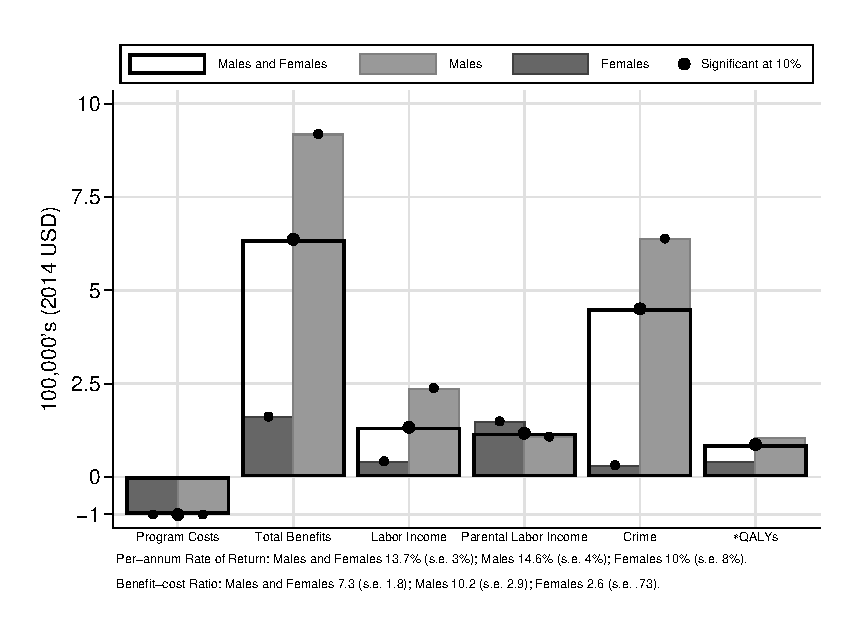
\includegraphics[width=.7\columnwidth]{output/abccare_npvssumm.eps}
\floatfoot{
\footnotesize
Note: This figure displays the life-cycle net present values of the main components of the cost/benefit analysis of ABC/CARE from birth to age 79, discounted to birth at a rate of 3\%.  By ``net" we mean that each component represents the total value for the treatment group minus the total value for the control group. Program costs: the total cost of implementing ABC/CARE. Total net benefits: the total net benefits of \textit{all} the components we consider. Labor income: total individual labor income from ages 20 to the retirement of program participants. Parental income: total parental labor income of the parents of the program participants from when the participants were ages 0 to 15. Crime: the total cost of crime (judicial and victimization costs). Total medical costs: both private and public medical costs from ages 15 to 79. Costs of education: the total costs of education of the individual from ages 6 to 26 and include any costs from special education and grade retention. \\
*QALYs refers to the quality-adjusted life years gain due to better health conditions through age 79.}
\end{sidewaysfigure}

The rest of the paper justifies and interprets these estimates. We proceed in the following way. Section~\ref{section:background} discusses main features of ABC/CARE. Section~\ref{section:methodsquestions} discusses the methodological challenges faced in evaluating the program.

We use three main approaches for characterizing the program's multiple lifetime benefits. We estimate treatment effects of ABC/CARE, accounting for multiple hypothesis testing by adjusting $p$-values for the multiplicity of reported outcomes to avoid cherry-picking of ``significant'' results;\footnote{\cite{Romano_Wolf_2005_JASA}. For an application, see, e.g., \cite{Heckman_Moon_etal_2010_QE}.} we also estimate combining functions that summarize the \emph{number} of beneficial outcomes (as well as the number of statistically significant beneficial outcomes) within blocks of outcomes and overall. Section~\ref{section:methodology} discusses these different approaches to inference. Section~\ref{section:cbamethodology} discuss our principal approach, cost/benefit and rate of return analysis, in which we monetize the costs and benefits associated with all of the outcomes.

A major methodological challenge is control group substitution bias.\footnote{See \cite{Heckman_1992_randomization}, \cite{Heckman_Hohmann_etal_2000_QJE}, and \cite{Kline-Walters_2016_QJE}.} Roughly 70\% of our experimental control groups take some form of alternative preschool at least some of the time. We define and estimate counterfactuals accounting for substitution bias that correspond to (i) treatment versus the next best option, (ii) treatment versus staying at home, and (iii) treatment versus attending an alternative preschool.

Section~\ref{section:results} presents our estimated treatment effects and combining functions. Section~\ref{section:cbaresults} presents our results from the cost/benefit and rate of return analysis. Estimates from different approaches agree. There are substantial benefits that differ by gender. In terms of treatment effects, women benefit across more of our measured domains. However, the monetized value of the treatment effects is greater for men. This discrepancy is largely driven by the health benefits and reduced crime for males. Section~\ref{section:conclusion} concludes.

\section[Background and Data Sources]{Background and Data Sources} \label{section:background}

\subsection{Overview}

ABC/CARE targeted disadvantaged children in Chapel Hill/Durham, North Carolina.\footnote{Both ABC and CARE were designed and implemented by researchers at the Frank Porter Graham Center of the University of North Carolina in Chapel Hill.} Table~\ref{tab:programcomparison} presents an overview and compares the two programs. Here, we summarize its main features. Appendix~\ref{appendix:background} describes these programs in detail.

The goals of the intervention were to enhance the early-life skills of a disadvantaged population. The intervention (i) supported language, motor, and cognitive development; (ii) minimized high-risk behaviors; and (iii) developed socio-emotional competencies considered crucial for school success including task-orientation, competence in communications, independence, and pro-social behavior.\footnote{\citet{Ramey_Collier_etal_1976_CarolinaAbecedarianProject, Ramey_etal_1985_Project-CARE_TiECSE, Sparling_1974_Synth_Edu_Infant_SPEECH, Wasik_Ramey_etal_1990_CD, Ramey-etal_2012-ABC}.}

The program provided individualized treatment. Each child's progress was recorded and learning activities were appropriately adapted every 2 to 3 weeks. Environments were organized to promote pre-literacy and access to a rich set of learning tools.\footnote{The ``Learningames'' approach was implemented by infant and toddler caregivers in 1:1 child-adult interactions. Each ``Learningames'' activity stated a developmentally-appropriate objective, the necessary materials, directions for teacher behavior, and expected child outcome.} The curriculum emphasized active learning experiences, dramatic play, and basic ideas of order and category (``pre-academic skills''), as well as discipline and the ability to interact with and respect others.  At later ages (3 through 5), the program became increasingly structured, focusing on the development of ``socio-linguistic and communicative competence.''\footnote{\citet{Ramey-et-al_1977_Intro-to-ABC, Haskins_1985_CD, Ramey_1981_Modification, Ramey_Campbell_1979_SR, Ramey_Smith_1977_AJMD, Ramey_McGinness_etal_1982_Abecedarianapproach, Sparling_Lewis_1979_BOOKLearninggamesFirstThree,Sparling_Lewis_1984_BOOKLearningGamesThreesFours}.}

ABC recruited four cohorts of children born between 1972 and 1976. CARE recruited two cohorts of children, born in 1978 and 1979. The recruitment processes for each study were identical. Potential participant families were referred to researchers by local social service agencies and hospitals at the beginning of the mother's last trimester of pregnancy. Eligibility was determined by a score of 11 or above on a High-risk Index (HRI).\footnote{See Appendix~\ref{appendix:background} for details on the construction of the HRI. Maternal education, family income, and father's job stability are major ingredients.}

As shown in Table~\ref{tab:programcomparison}, the design and implementation of both ABC and CARE were similar. ABC had two phases, the first of which lasted from birth until age 5. In this phase, children were randomly assigned to either a treatment group that received center-based childcare or a control group. The second phase of treatment consisted of academic support from ages 5 through 8. CARE consisted of two treatment phases that were very similar to those of ABC. The first phase of CARE, also lasting from birth until age 5, contained an additional treatment arm, family education, designed to study the effects of improving the home environment on child development.\footnote{\citet{Wasik_Ramey_etal_1990_CD}.}

Our analysis pools the treatment group in CARE that received the center-based ABC curriculum with the ABC treatment group. We do not use the data on the CARE treatment group that only received family education.\footnote{\citet{ABCCARE_Dataset} show that there is no effect of the CARE family education component alone.} We only consider the intervention through age 5.\footnote{The second-phase treatment of ABC/CARE had very weak, if any, effects (\citealp{Campbell_Conti_etal_2014_EarlyChildhoodInvestments} and \citealp{ABCCARE_Dataset}).}

\begin{table}[htbp]
\centering
\caption{ABC and CARE, Program Comparison} \label{tab:programcomparison}
\begin{adjustbox}{max width=\textwidth}
\begin{threeparttable}
	\input{output/abccare_programcomparison_2016-08-27a_alz.tex}
\begin{tablenotes}
\footnotesize
\item Note: This table compares the main elements of ABC and CARE, summarized in this section. A \checkmark\ indicates that ABC and CARE had the same characteristic.
\end{tablenotes}
\end{threeparttable}
\end{adjustbox}
\end{table}

For both programs, from birth until the age of 8, data were collected annually on cognitive and socio-emotional skills, home environment, family structure, and family economic characteristics. After age 8, data on cognitive and socio-emotional skills, education, and family economic characteristics were collected at ages 12, 15, 21, and 30.\footnote{At age 30, measures of cognitive skills are unavailable for both ABC and CARE.} In addition, we have unique administrative criminal records and a full medical survey at age 34. This allows us to study the long-term effects of the programs along multiple dimensions of human development.\footnote{See Appendix~\ref{appendix:data} for a more comprehensive description of the data. In Appendix~\ref{appendix:randomization}, we document the balance in observed baseline characteristics across the treatment and control groups, once we drop the individuals for whom we have crime or health information, for which there is substantial attrition. Further, the methodology we propose addresses missing information in either of these two outcome categories.}

\subsection{Randomization Protocol and Compromises} \label{section:randomization}

Randomization for both ABC and CARE were conducted at the family level. Pairs of siblings and twins were jointly randomized into either treatment or control groups.\footnote{Sibling pairs occurred when the two siblings were close enough in age such that both of them were eligible for the program.} Although we know that pairing was based on HRI, maternal IQ, maternal education, maternal age, and gender of the subject, we do not know the original pairs. ABC collected an initial sample of 122 subjects. 22 subjects did not complete the first-phase of treatment as initially assigned by the randomization. We characterize each of the cases in Appendix~\ref{appendix:assessingcc} and document that our estimates are robust when we adjust for missing data using  standard methods.\footnote{In Appendix~\ref{appendix:methodology}, we compare the observed, baseline characteristics of the subjects in Table~\ref{table:abccompromises} to the observed, baseline characteristics of the subjects who complied to the initial treatment assignment. We find little evidence of differences.}

\subsection{Control Group Substitution}

In ABC/CARE, many control group members attended alternative preschools.\footnote{See \cite{Heckman_Hohmann_etal_2000_QJE} on the issue of substitution bias on social experiments.} In ABC, \treatsubsabc\ of control-group subjects were enrolled in one of 11 local center-based childcare centers. In CARE, \treatsubscarec\ of the control group were enrolled in alternative preschools. Figure~\ref{fig:treatsubcare}a shows (for each program) the cumulative distribution of the proportion of time control subjects were enrolled in alternative preschool from birth to age 5. Figure~\ref{fig:proportion-alt-pre}b shows the distribution of time spent in the alternative program for control group participants and Figure~\ref{fig:enrollment-by-age}c shows the same thing for each age between birth and 5.

Most of the alternative preschools received federal subsidies and were subject to federal regulations.\footnote{See \citet{Department-of-Health_1968_DayCareRequirements,NCGA_1971_House-Bill-100,Ramey-et-al_1977_Intro-to-ABC,Ramey_Campbell_1979_SR,Ramey_McGinness_etal_1982_Abecedarianapproach, Burchinal_Campbell_etal_1997_CD}.} Child caregivers were required to be trained in early childhood education. The centers were required to implement an approved curricula designed to enhance cognitive, social, and linguistic competence in disadvantaged children.\footnote{\citet{Burchinal_etal_1989_CD_Daycare-Pre-K-Dev}.}

\begin{sidewaysfigure}[H]
\caption{Control Substitution Characteristics, ABC/CARE Control Group}\label{fig:control-sub}
\begin{center}
\begin{tabular}{cc}
(a) Enrollment & (b) Enrollment Intensity\\
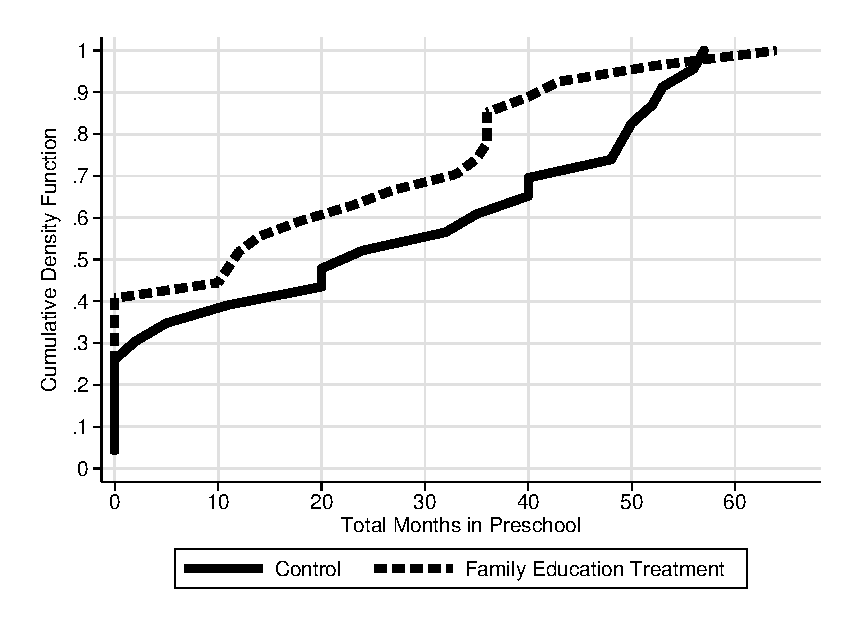
\includegraphics[width=.45\textwidth]{output/care_controlcontamination_months.eps}\label{fig:treatsubcare} &
\includegraphics[width=.45\textwidth]{output/abccare_Vfractimes.eps}\label{fig:proportion-alt-pre}
\end{tabular}\\
(c) Enrollment by Age\\
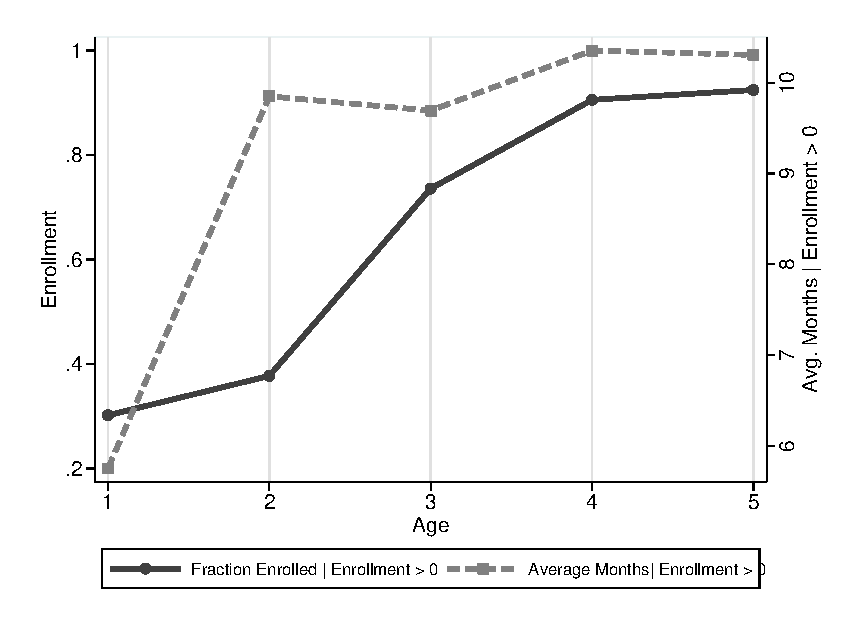
\includegraphics[width=.45\textwidth]{output/abccare_Valtenrollment.eps}\label{fig:enrollment-by-age}
\end{center}
\begin{tablenotes}
\item Note: Panel (a) displays the cumulative distribution function of enrollment in alternative preschools of the ABC/CARE control group. Panel (b) displays the fraction of children in the ABC/CARE control group enrolled in alternative preschool during the fraction of months from ages 0 to 5 (conditional on ever being enrolled) in the $x$-axis. Panel (c) displays enrollment in alternative preschools of ABC/CARE control group by age in the left axis and average number of months in alternative preschool conditional on enrollment by age in the right axis.\\
\end{tablenotes}
\end{sidewaysfigure}

\section{Parameters of Interest and Policy Questions} \label{section:methodsquestions}

Random assignment to treatment does not guarantee that conventional treatment-effect estimates answer policy-relevant questions. We define and use three parameters that address different policy questions.

Let $Y$ denote an outcome of interest. $D=1$ indicates that parents agree to participate in the program.\footnote{Parameters are defined as conditional on parents agreeing to participate in the program, i.e., conditional on $D = 1$. We find little sensitivity to the few cases of non-compliance in Appendix~\ref{appendix:assessingcc} and adjust our estimates for the cases of attrition as we explain in Appendix~\ref{appendix:attrition}.} $R | D = 1$ indicates randomization to either treatment or control status for those who agree to participate. $T$ denotes periods during the first phase of treatment---$T \in \left\{ 0,\dots,5 \right\}$. We consider two relevant counterfactual states for control groups. Individual subscripts are omitted for simplicity:
\begin{eqnarray}
Y_H^0\left(t \right) &:& \textbf{ Subject stays at home in time period $t$} \nonumber \\
Y_C^0\left(t \right) &:& \textbf{ Subject attends alternative preschool in time period $t$}.  \nonumber
\end{eqnarray}

We simplify the analysis by assuming that timing of receipt of childcare in the first five years is irrelevant for the realization of the outcome:\footnote{Describing the dynamic choices underlying $V$ is of interest but goes beyond the scope of this paper.}
\begin{align}
Y_H^0 \left( t \right) &= Y_H^0 \nonumber \\
Y_C^0 \left( t \right) &= Y_C^0.
\end{align}

Let $V$ indicate the fraction of time spent in an alternative preschool. The counterfactual outcome when a child is in control status is
\begin{equation}
Y^0 : = \left( 1 - V \right) Y_H^0 + \left( V \right) Y_C^0.
\end{equation}

Our analysis abstracts from the dynamics of $V$ and the associated dynamic outcomes.\footnote{We treate $V$ as binary.} Ideally, we would construct the counterfactual $Y_C^0 \left( V \right)$ specific to each realization of $V \in [0,1]$. However, this is empirically infeasible in light of the small number of observations available to us. We break $V$ into two categories, $V=0$ and $V>0$.

Our first parameter addresses the question: what is the effect of the program as implemented? i.e, what is the effect of the program without fixing the parental decision to enroll the subject in alternative preschool? This parameter is $\Delta := \mathbb{E} \left[ Y^1 -  Y_0 | D =1 \right]$. It addresses the effectiveness of the program relative to the quality of alternative preschools in place when the program was implemented.

Random assignment to either the treatment or control group allows us to identify this parameter.

It is also fruitful to ask: what is the effectiveness of the program with respect to a counterfactual world in which the child stays at home? The associated causal parameter is:
\begin{equation}
\Delta \left(V = 0 \right) : =   \mathbb{E} \left[ Y^1 \left( V \right) - Y^0 \left( V \right) | V = 0, D = 1 \right]. \label{eq:par0}
\end{equation}
Random assignment to the treatment group does not directly identify this parameter.

The average effectiveness of a program relative to the attendance in alternative preschool is:
\begin{equation}
\Delta \left( V > 0 \right) : =   \mathbb{E} \left[ Y^1 \left(V \right) - Y^0 \left( V \right) | V > 0, D = 1 \right] \label{eq:par1}
\end{equation}

\section{Inference} \label{section:methodology}

\subsection{Sample Size}

Evidence from ABC/CARE and other early childhood programs has been criticized because of its small sample size.\footnote{See, e.g., Murray in \cite
{Heckman_2013_BOOKGivingkidsfair}.} An extensive analysis by \citet{Campbell_Conti_etal_2014_EarlyChildhoodInvestments} shows that asymptotic inference and small sample-based permutation-based inference closely agree. We use large sample inference in this paper.\footnote{Inference based on permutation tests is available on request.}

\subsection{Summarizing Vectors of Treatment Effects: Stepdown Tests and Combining Functions}  \label{section:counts}

This paper focuses on mean treatment effects of the program on multiple dimensions of human development. We have measures of outcomes from very early in life to the mid-30s. Summarizing these effects in a meaningful way is a challenging task. We present stepdown $p$-values for blocks of outcomes that are used in our cost/benefit analysis.\footnote{\citet{Lehman_Romano_2005_AnnStat,Romano_Shaikh_2006_AnnStat}.} We also summarize our data using simple combining functions that count the proportion of treatment effects that category that show beneficial outcomes.

Consider a block of outcomes indexed in $B_l$. Let $\# B_l$ denote the number of interpretable of outcomes in the block. Let $j \in B_l$ be a particular outcome within the block. Associated with it is a mean treatment effect

\begin{equation}
\Delta_j : = E(Y^1_j - Y^0_j | \Delta=1).
\end{equation}

We assume that outcomes can be evaluated so that $\Delta_j >0$ is beneficial.\footnote{All but 5\% of the outcomes we study can be ranked in this fashion.} We summarize the effect of the program on outcomes within the block by

\begin{equation}
T_l = \displaystyle\sum^{\# B_l}_{j=1} 1 (\hat{\Delta}_j >0).
\end{equation}

\noindent i.e., we count the number of beneficial outcomes within each block. The proportion of beneficial outcomes is $T_l / \# B_l$.

Under the null hypothesis of no treatment effects for all $j \in B_l, l \in \mathcal{L}$, the number of blocks, and assuming the validity of asymptotic approximations, $T_l / \# B_l$ should be centered around $Y_2$. We bootstrap to obtain a $p$-value for the null for each block and overall blocks.

Alternatively, we also count the individually beneficial treatment effects which are statistically significant in the sets of outcomes across each of the groups indexed by the set $B_l$. Using a 10\% significance level, on average 10\% of all outcomes should be ``significant'' at the 10\% level even if there is no treatment effect of the program.

Using a combing function across all blocks enables us to avoid (i) arbitrarily picking outcomes that have statistically significant effects---``cherry picking''; or (ii) arbitrarily blocking sets of outcomes to correct the $p$-values when accounting for multiple hypothesis testing.

\section{Forecasting and Monetizing Life-cycle Costs and Benefits} \label{section:cbamethodology}

Benefit-cost analysis requires forecasting the benefits of the program over the entire life cycle. This section explains our strategy for interpolating and extrapolating the life-cycle costs and benefits of education, labor income, crime, and health.\footnote{The methodology for doing this exercise for public-transfer income is analogous to that of labor income so we suppress the description for brevity.} A variety of important practical issues are discussed in Appendix~\ref{appendix:methodology}, in which we also explain a solution for cases of attrition when forecasting.

\subsection{Education}

Follow-up data on educational attainment were collected up to age 30. In Appendix \ref{appendix:education}, we show that education up to this age is an accurate portrayal of lifetime educational attainment. Therefore, we do not forecast beyond age 30. To monetize the costs of education, we consider the public costs of K-12 education and the private costs of post-secondary education, including vocational programs and community college. Other costs of education include grade retention and special education.

\subsection{Labor Income}

We observe labor income at ages 21 and 30. To construct life-cycle profiles, we interpolate between ages 21 and 30 and extrapolate from ages 31 to 67, at which age we assume subjects retire. Recall that $R$ indicates whether the subject was randomized to the treatment group ($R=1$) or to the control group ($R=0$), conditional on having agreed to participate in the program ($D = 1$). $Y$ is the outcome for which we want to produce a forecast---interpolation or extrapolation. In this case, the outcome is labor income. $X$ is a vector of observed characteristics, possibly affected by the treatment---e.g. lagged values of $Y$; $W$ is a vector of baseline characteristics---e.g. race and gender; $S$ indicates whether we observe $Y$ in the experimental sample ($S=1$) or an auxiliary, non-experimental data source ($S=0$). For simplicity, we suppress $D$ and individual and time subscripts. \\

We aim to forecast

\begin{equation}
Y = \phi \left( R, X, W, S \right) + \varepsilon \label{eq:forecast-param}
\end{equation}

\noindent where we assume that the outcome of interest is an additively separable function of the known objects $R, X, W, S$ and an unobserved component $\varepsilon$.

Identifying $\phi \left( R, X, W, S \right)$ requires some assumptions. Because the forecast is based on observed characteristics, $X$, we require the auxiliary datasets to share the support on observed characteristics with the experimental dataset:

\begin{equation}
\sup \left( X | S = 1 \right) \subseteq \sup \left( X | S = 0 \right).
\end{equation}

Given that we are not able to observe $R$ in the auxiliary dataset, we assume that we are able to summarize the impacts that the treatment has on the outcomes with observed characteristics. That is, we are assuming the conditional independence and sufficiency of $S, X$, and $W$ to describe treatment. Formally, let the $^{*}$ superscript denote variables we do not observe. In the auxiliary dataset we have: $\left( S = 0, Y, X, W, R^* \right)$. In the experimental dataset we have: $\left( S = 1, Y^*, X, W, R \right)$. This assumption can be written as:

\begin{equation}
\mathbb{E} \left[ Y | R = r, X = x, W = w, S = s\right] =  \mathbb{E} \left[ Y | X = x^r, W = w, S = s\right]
\end{equation}

\noindent where $x^r$ is a draw from the distribution of $X | R = r$.

To be able to fully ``link'' the individuals in the auxiliary data set with those in the experimental datasets to produce forecasts, we must make a similar assumption. We assume that we can summarize the difference between the individuals in the experimental datasets and those in the auxiliary datasets based on observed characteristics. This conditional independence and sufficiency of $X, W$, and $R$ to describe the presence of an individual in the data is written formally as:

\begin{equation}
\mathbb{E} \left[ Y^* | R = r, X = x, W = w, S = 1 \right] = \mathbb{E} \left[ Y | R^* = r , X = x, W = w, S = 0\right].
\end{equation}

These assumptions allow us to compute the estimator of \eqref{eq:forecast-param}:

\begin{equation}
\widehat{Y} = \widehat{\phi} \left( R, X, W, S = 1 \right) + \widehat{\varepsilon},   \label{eq:additive}
\end{equation}

\noindent where $\phi \left( R, X, W, S \right) : = \mathbb{E} \left[ Y | R = r, X = x, W = w, S = s \right] $ and $\widehat{\varepsilon}$ is a forecasting error.

These assumptions imply that

\begin{equation}
\phi \left( R, X, W, S = 1 \right) = \mathbb{E} \left[ Y | X = x^r, W = w, S = 0 \right]
\end{equation}

\noindent where $\mathbb{E} \left[ Y | X = x^r, W = w, S = 0 \right]$ is a moment in the auxiliary dataset. The estimation of $\mathbb{E} \left[ Y | X = x^r, W = w, S = 0 \right]$ produces a residual of the form $\widehat{\varepsilon} : = Y - \widehat{Y}$ for each individual. The forecast for each  individual outcome consists of $\widehat{\phi} \left( \cdot \right)$ and a draw from the empirical distribution of $\widehat{\varepsilon}$, which we call forecast error. We account for this error when interpolating and extrapolating the crime and health outcomes in addition to income.

\subsection{Crime}  \label{sec:crime}

To estimate the life-cycle benefits and costs of ABC/CARE related to criminal activity, we use rich data on crime outcomes.\footnote{Two previous studies consider the impacts of ABC on crime: \citet{Clarke_Campbell_1998_ABC_Comparison_ECRQ} use administrative crime records up to age 21, and find no significant differences between the treatment and the control groups. \cite{Barnett_Masse_2007_EER} mention crime in their cost-benefit analysis, but they cite the previous study to claim that there are no savings coming from a reduction in crime.} See Appendix \ref{appendix:crime} for a more complete explanation of the following procedures.

We consider the following types of crime: arson, assault, burglary, fraud, larceny, miscellaneous (which includes traffic and non-violent drug crimes), murder, vehicle theft, rape, robbery, and vandalism. We use administrative data that detail: (i) youth arrests, gathered at the age-21 follow-up; (ii) adult arrests, gathered at the age-34 follow-up; and (iii) sentences, gathered at the age-34 follow-up. We also use self-reported data on adult crimes, gathered in the age-21 and age-30 subject interviews. Because none of these sources capture all criminal activity, it is necessary to combine them to more completely approximate the crimes the subjects committed. We also use several auxiliary datasets to complete the life-cycle profile of criminal activity and compute the costs of the committed crimes

We follow four steps to estimate the costs of crime.

\begin{enumerate}
\item \textit{Count arrests and sentences.} We start by counting the total number of sentences for each individual and type of crime (arson, assault, etc.) up to age 34, matching crimes across data sources, to construct the total number of  arrests for each individual and type of crime up to age 34.\footnote{In practice, we count all offenses (an arrest might include multiple offenses). This gives the correct number of victims for our estimations. The youth data have coarser categories than the rest of the data: violent, property, drug, and other. To match these data with the adult data, we assume that all property crimes were larcenies and that all violent crimes are assaults. In the ABC/CARE sample, assault is the most common type of violent crime, and larceny/theft is the most common property crime.} For individuals missing arrest data,\footnote{About 10\% of the ABC/CARE sample has missing arrest data.} we impute the number of arrests by multiplying the number of sentences for each type of crime by a national arrest-sentence ratio for the respective crime.\footnote{This arrest-sentence ratio is constructed using the National Crime Victimization Survey (NJRP) and and the Uniform Crime Reporting Statistics (UCRS).}

\item \textit{Construct predictions.} Based on the sentences observed before age 34, we predict the sentences that the ABC/CARE subjects will have after age 34. Data from the North Carolina Department of Public Safety (NCDPS), which provide lifetime sentences of individuals in North Carolina, are used to estimate sentences incurred after age 34 from sentences incurred before age 34. Applying these models to the ABC/CARE data, we predict the number of future sentences for each subject up to age 50.\footnote{We assume that individuals with no criminal records before age 34 commit no crimes after age 34.} We then add these estimates to the original number of sentences, getting an estimate of the lifetime sentences. Adding these estimates increases the total count of crimes by 30\%--50\%.

\item \textit{Estimate number of victims from the crimes.} We only observe crimes that resulted in consequences in the justice system: crimes that resulted in arrests and/or sentences. To include unobserved crimes, we use victimization inflation (VI).\footnote{Previous papers using this method include \citet{Belfield_Nores_etal_2006_JHR} and \cite{Heckman_Moon_etal_2010_RateofReturn}.} We start by constructing a VI ratio, which is the national ratio of victims and arrests for each type of crime.\footnote{We assume that each crime with victims is counted separately in the national reports on arrests, even for arrests that might have been motivated by more than one crime. This victim-arrest ratio is constructed using the NJRP and the National Crime Victimization Survey (NCVS).} Then, we estimate the number of victims from the crimes committed by ABC/CARE subjects as their total arrests multiplied by the VI ratio.\footnote{Additionally, we can calculate an analogous estimate of the number of crime victims using sentences, based on the VI ratio and the national arrests-to-sentences ratio. Both estimates are very similar, as shown in Appendix \ref{appendix:crime}. To improve precision, the estimates in the rest of our paper are based on the average of the two calculations.}

\item \textit{Find total costs of crimes.} We use the estimates of the cost of crimes for victims from \cite{McCollister_etal_2010_DAD} to impute the total victimization costs. For crimes resulting in arrests and/or sentences, we consider justice system costs as well, such as police costs.\footnote{To be able to assign costs to each type of crime, we assume that the cost of the justice system depends on the number of offenses of each type, rather than on the number of arrests. While this could very slightly overestimate justice system costs, the costs only represent about 5\% of the total crime costs.} Finally, we construct the total costs of incarceration for each subject using the total prison time and the cost of a day in prison.
\end{enumerate}

\subsection{Health} \label{section:health}

To forecast and monetize health outcomes, we consider three issues: (i) health outcomes such as diabetes or heart disease are absorbing states; (ii) health outcomes are highly interdependent within and across time periods; and (iii) there is no evident time period available to finish accounting for benefits and costs.\footnote{For example, for income we extrapolate up to the retirement age of 67. However, for health, we need to predict an age of death for each individual.} It is not sufficient to condition on observed characteristics to recover a credible estimate of the treatment effect. Instead, we use an adaptation of the Future America Model (FAM) that projects health outcomes from the subjects' mid-30s up to their projected death \citep{Goldman_etal_2015_Future-Elderly-Model-Report}.\footnote{The simulation starts at the age in which we observe the subject's age-34 health follow-up. On average this happened at age 34 for both males and females, but there is variation ranging from age 30 to age 37.} Appendix~\ref{appendix:health} discusses the FAM methodology.

The methodology has six steps: (i) estimate age-by-age health state transition probabilities using the Panel Study of Income Dynamics (PSID); (ii) match these transition probabilities to the ABC/CARE subjects based on observed characteristics; (iii) estimate quality-adjusted life year (QALY) models using the Medical Expenditure Panel Survey (MEPS) and the PSID; (iv) estimate medical cost models using the MEPS and the Medicare Current Beneficiary Survey (MCBS), allowing estimates to differ by health state and observed characteristics; and (v) predict the medical expenditure and QALYs that correspond to the simulated individual health trajectories.\footnote{As an intermediate step between (i) and (ii), we impute some of the variables used to initialize the FAM models (see Appendix~\ref{appendix:health}).}

Our microsimulation model starts the health predictions at age 30, with the information on observed characteristics available at this age. Restricting it to the individuals for whom we have information from the age-34 health follow-up allows us to account for components that are crucial for predicting health outcomes, such as the body mass index (BMI). The models predict the probability of being in any of the states in the horizontal axis of Table~\ref{table:transition} at age $a+1$ based on the state at age $a$, which is described by the vertical axis of the table.\footnote{In practice, the predictions are based on two-year lags, due to data limitations in the auxiliary sources we use to simulate the FAM. For example, if the individual is 30 (31) years old in the age-30 interview, we simulate the trajectory of her health status at ages 30 (31), 32 (33), 34 (35), and so on until her projected death.} Absorbing states are an exception. For example, heart disease at age $a$ does not enter in the estimation of transitions for heart disease at age $a+1$ because it is an absorbing state: once a person has heart disease, she carries it through the rest of her life.\footnote{The same is true for chronic or permanent conditions such as hypertension, having a stroke, etc.}

At each age, once we obtain the transition probability for each health outcome, we draw a Monte-Carlo simulation for each subject. Thus, each simulation depends on each individual's health history and on their particular characteristics. For every simulated trajectory of health outcomes, we predict the lifetime medical expenditure using the models estimated from the MEPS and the MCBS. We then obtain an estimate of the expected lifetime medical expenditure by taking the mean of each individual's simulated lifetime medical expenditure.

The same procedure is applied to calculate quality-adjusted life years (QALYs).\footnote{A quality-adjusted life year (QALY) reweighs a year of life according to its quality given the burden of disease. A QALY of 1 denotes a year of life in the absence of disease (perfect health). The value of QALY for an individual in a given year is smaller than 1 when there is positive burden of disease, as worse health conditions imply lower QALYs. When an individual dies, her QALY equals zero. It is worth noting that there are extreme combinations of disease and disability that may generate negative QALYs, although this case is unusual.} We compute a QALY model based on the EQ-5D instrument, a widely-used Health-related Quality-of-life (HRQoL) measure, available in MEPS. We then estimate this model from the PSID.

\begin{sidewaystable}[H]
\begin{threeparttable}
\caption{Health State Transitions, Age $a$ as Predictor of Age $a+1$}\label{table:transition}
\scriptsize
\begin{tabular}{l|ccccccccccccccc} \hline \hline 
\multicolumn{1}{c}{Age $a$} & \multicolumn{15}{c}{Age $a+1$} \\ \hline
  & Heart & Hypertension & Stroke & Lung Disease & Diabetes & Cancer & Disability & Mortality & Smoking & Obesity & Health  & DI  & SS  & DB  & SSI  \\
&  Disease &  &  & Disease & & & & &  &  & Insurance & Claim & Claim & Claim & Claim \\
Heart Disease & & & $\times$& & & &$\times$ &$\times$ &$\times$ &     $\times$        &  $\times$      &  $\times$  & $\times$ & $\times$ & $\times$\\
Hypertension  & & & $\times$ & & & &$\times$ &$\times$ &$\times$ &         $\times$    &   $\times$    & $\times$   & $\times$ & $\times$ & $\times$ \\
Stroke           & & & & & & &$\times$ &$\times$ &$\times$ &       $\times$       &     $\times$   &   $\times$  & $\times$ & $\times$ & $\times$ \\
Lung Disease & & & & & & &$\times$ &$\times$ & $\times$&       $\times$      &   $\times$     &   $\times$  &$\times$  & $\times$ & $\times$ \\
Diabetes       & $\times$ &$\times$  & &  $\times$ & & &$\times$ &$\times$ & $\times$&         $\times$    &   $\times$     &  $\times$   & $\times$ & $\times$ & $\times$ \\
Cancer         & & & &  $\times$ & & &$\times$ & $\times$& $\times$&     $\times$       &   $\times$      &   $\times$  & $\times$ & $\times$ & $\times$ \\
Disability     & & & & & & &$\times$ &$\times$ & $\times$&     $\times$       &    $\times$     &     $\times$  & $\times$ & $\times$ & $\times$ \\
\hline
DI Claim      & & & & &  & & & & &            &    $\times$     & $\times$      & $\times$ & $\times$ & $\times$ \\
SS Claim     & & & & & & & & &           &         &    $\times$  & & & $\times$ & $\times$\\
DB Claim    & & & & &&  & & & &         &        &      & $\times$ & & $\times$ \\
SSI Claim   & & & & &&  & & & &         &        &      & & & $\times$ \\ \hline \hline
\end{tabular}
\begin{tablenotes}
\footnotesize
\item Note: This table illustrates how health outcomes at age $a$ predict health outcomes at age $a+1$. The crosses indicate if we use the age $a$ outcome to predict the age $a+1$ outcome. DI Claim: disability insurance claim; SS Claim: social security claim; DB Claim: disability benefits claim; SSI Claim: supplemental security income claim. The age $a$ states that do not predict themselves at age $a+1$ are absorbing states by construction.
\end{tablenotes}
\end{threeparttable}
\end{sidewaystable}

We estimate three models of medical spending: (i) Medicare spending (annual medical spending paid by parts A, B, and D of Medicare); (ii) out-of-pocket spending (medical spending paid directly by the individual); and (ii) all public spending other than Medicare. Each medical spending model is estimated through pooled weighted least squares regressions that include a person's demographics, economic status, current health, risk factors, and functional status as explanatory variables. The MCBS-based medical spending models also include lagged health because of the length of time for which MCBS subjects are observed.

We also calculate medical expenditure before age 30. We combine the MEPS and retrospective information in the ABC/CARE interviews at ages 21 and 30 related to hospitalizations at ages 12 and 15 and births at age 15. In addition to this retrospective information, we use use individual and family demographics to predict medical expenditure models for each age.

The first level of each model predicts the likelihood that the subject incurred any medical expenditure in the period. The second level predicts the medical expenditure for those with positive expenditures.

\section{Empirical Estimates}\label{section:results}

\subsection{Treatment Effects}\label{section:teresults}

An overview of treatment effects is given in Tables~\ref{resultsfemales} and \ref{resultsmales}. Appendix~\ref{appendix:results} gives the complete list of mean treatment effects displays an extensive summary. We select these outcomes because we consider them of economic interest.\footnote{Appendix~\ref{appendix:results} displays results accounting for multiple hypothesis testing as in \citet{Lehman_Romano_2005_AnnStat} and \citet{Romano_Shaikh_2006_AnnStat}. We do not lose significance in the main outcomes driving the cost/benefit analysis.}

The results for females indicate an increase in employment, which strengthens when comparing to the females who did not receive alternative preschool. Females in the treatment group were more likely to graduate from high school and receive more years of education than those in the control group. These education results are robust even after fixing the take-up of alternative preschool.

The robust results for males are in health outcomes as opposed to education outcomes. Treated subjects reported lower drug use and blood pressure. The results for employment, hypertension, blood pressure, and graduation from a 4-year college are strengthened when fixing the control group to those subjects who attended alternative preschools. This is an opposite pattern from the results of the females.

\begin{table}[H]
\centering
\begin{threeparttable}
\caption{Selected Outcomes, ABC/CARE Females}\label{resultsfemales}
\begin{scriptsize}
\input{output/select_rslt_female_2016-08-26a_alz}
\end{scriptsize}
\begin{tablenotes}
\footnotesize
\item Note: This table shows the treatment effects for categories outcomes that are important for our cost/benefit analysis. Systolic and Diastolic blood pressure are measured in terms of mm Hg. Bootstrapped $p$-values are in parentheses. (1) Mean difference between the groups randomly assigned to receive center-based childcare and the groups randomly assigned not to. (2) Adjusts estimates in (1) for attrition and controls for a set of covariates. (3) Mean difference between the groups randomly assigned to received center-based childcare and the groups randomly assigned not to, restricting the latter to subjects who did not receive preschool alternatives. (4) Mean difference between the groups randomly assigned to received center-based childcare and the groups randomly assigned not to, placing a relatively high weight to the subjects who are likely not to be enrolled in alternative preschools. (5) Mean difference between the groups randomly assigned to received center-based childcare and the groups randomly assigned not to, restricting the latter to subjects received preschool alternatives. (6) Mean difference between the groups randomly assigned to received center-based childcare and the groups randomly assigned not to, placing a relatively high weight to the subjects who are likely to be enrolled in alternative preschools.
\end{tablenotes}
\end{threeparttable}
\end{table}


\begin{table}[H]
\centering
\begin{threeparttable}
\caption{Selected Outcomes, ABC/CARE Males}\label{resultsmales}
\begin{scriptsize}
  \begin{tabular}{ccccccccccc}
  \toprule
   Category & Variable & Age & (1) & (2) & (3) & (4) & (5) & (6)\\
    \midrule
    % cat 7
     \mc{1}{l}{Labor Income} & \mc{1}{l}{Employed} & \mc{1}{c}{30} & \mc{1}{c}{0.119} & \mc{1}{c}{0.179} & \mc{1}{c}{-0.050} & \mc{1}{c}{0.041} & \mc{1}{c}{0.245} & \mc{1}{c}{0.262} \\

     & &  & \mc{1}{c}{\textbf{(0.079)}} & \mc{1}{c}{\textbf{(0.039)}} & \mc{1}{c}{(0.579)} & \mc{1}{c}{(0.355)} & \mc{1}{c}{\textbf{(0.013)}} & \mc{1}{c}{\textbf{(0.000)}} \\

    &   \mc{1}{l}{Labor Income} & \mc{1}{c}{30} & \mc{1}{c}{19,810} & \mc{1}{c}{24,902} & \mc{1}{c}{21,069} & \mc{1}{c}{24,012} & \mc{1}{c}{28,483} & \mc{1}{c}{21,170} \\

   &  &  & \mc{1}{c}{\textbf{(0.079)}} & \mc{1}{c}{(0.171)} & \mc{1}{c}{(0.263)} & \mc{1}{c}{(0.105)} & \mc{1}{c}{(0.132)} & \mc{1}{c}{(0.158)} \\

    % cat 3
    \mc{1}{l}{Parental Income} &  \mc{1}{l}{Parental Income} & \mc{1}{c}{1.5} & \mc{1}{c}{330} & \mc{1}{c}{-97.199} & \mc{1}{c}{-2,384} & \mc{1}{c}{-1,168}  & \mc{1}{c}{-26.663} & \mc{1}{c}{872} \\

     & &  & \mc{1}{c}{(0.408)} & \mc{1}{c}{(0.461)} & \mc{1}{c}{(0.645)} & \mc{1}{c}{(0.632)} & \mc{1}{c}{(0.487)} & \mc{1}{c}{(0.329)} \\

   &  & \mc{1}{c}{3.5} & \mc{1}{c}{1,036} & \mc{1}{c}{223} & \mc{1}{c}{-1,152} & \mc{1}{c}{1,448} & \mc{1}{c}{47.496} & \mc{1}{c}{701} \\

   &  &  & \mc{1}{c}{(0.355)} & \mc{1}{c}{(0.500)} & \mc{1}{c}{(0.553)} & \mc{1}{c}{(0.395)}  & \mc{1}{c}{(0.447)} & \mc{1}{c}{(0.461)} \\

   &  & \mc{1}{c}{4.5} & \mc{1}{c}{821} & \mc{1}{c}{1,677} & \mc{1}{c}{3,815} & \mc{1}{c}{-2,662} & \mc{1}{c}{917} & \mc{1}{c}{-429} \\

    & &  & \mc{1}{c}{(0.355)} & \mc{1}{c}{(0.303)} & \mc{1}{c}{(0.132)} & \mc{1}{c}{(0.803)} & \mc{1}{c}{(0.434)} & \mc{1}{c}{(0.461)} \\

    % cat 8
      \mc{1}{l}{Crime} & \mc{1}{l}{Total Felony Arrests} & \mc{1}{c}{Mid-30s} & \mc{1}{c}{0.196} & \mc{1}{c}{0.683} & \mc{1}{c}{2.132} & \mc{1}{c}{1.337}  & \mc{1}{c}{0.466} & \mc{1}{c}{0.183} \\

   &  &  & \mc{1}{c}{(0.618)} & \mc{1}{c}{(0.711)} & \mc{1}{c}{(0.895)} & \mc{1}{c}{(0.974)}  & \mc{1}{c}{(0.645)} & \mc{1}{c}{(0.553)} \\

   & \mc{1}{l}{Total Misdemeanor Arrests} & \mc{1}{c}{Mid-30s} & \mc{1}{c}{-0.501} & \mc{1}{c}{-0.239} & \mc{1}{c}{0.085} & \mc{1}{c}{-0.040} & \mc{1}{c}{-0.343} & \mc{1}{c}{-0.512} \\

    & &  & \mc{1}{c}{(0.132)} & \mc{1}{c}{(0.316)} & \mc{1}{c}{(0.500)} & \mc{1}{c}{(0.395)}  & \mc{1}{c}{(0.224)} & \mc{1}{c}{(0.118)} \\

    % cat 9
      \mc{1}{l}{Health} & \mc{1}{l}{Self-reported drug user} & \mc{1}{c}{Mid-30s} & \mc{1}{c}{-0.333} & \mc{1}{c}{-0.432}  & \mc{1}{c}{-0.788} & \mc{1}{c}{-0.555}  & \mc{1}{c}{-0.326} & \mc{1}{c}{-0.330} \\

    & &  & \mc{1}{c}{\textbf{(0.026)}} & \mc{1}{c}{\textbf{(0.000)}} & \mc{1}{c}{\textbf{(0.000)}} & \mc{1}{c}{\textbf{(0.000)}} & \mc{1}{c}{\textbf{(0.053)}} & \mc{1}{c}{\textbf{(0.039)}} \\

    % cat 11
      & \mc{1}{l}{Systolic Blood Pressure} & \mc{1}{c}{Mid-30s} & \mc{1}{c}{-9.791} & \mc{1}{c}{-20.743} & \mc{1}{c}{16.605} & \mc{1}{c}{14.253} & \mc{1}{c}{-30.437} & \mc{1}{c}{-30.587} \\

     & &  & \mc{1}{c}{\textbf{(0.079)}} & \mc{1}{c}{\textbf{(0.000)}} & \mc{1}{c}{(0.908)} & \mc{1}{c}{(0.908)}  & \mc{1}{c}{\textbf{(0.000)}} & \mc{1}{c}{\textbf{(0.000)}} \\

  &  \mc{1}{l}{Diastolic Blood Pressure} & \mc{1}{c}{Mid-30s} & \mc{1}{c}{-10.854} & \mc{1}{c}{-19.895} & \mc{1}{c}{-12.199} & \mc{1}{c}{-8.150}  & \mc{1}{c}{-22.740} & \mc{1}{c}{-21.851} \\

    & &  & \mc{1}{c}{\textbf{(0.000)}} & \mc{1}{c}{\textbf{(0.000)}} & \mc{1}{c}{\textbf{(0.079)}} & \mc{1}{c}{\textbf{(0.026)}}  & \mc{1}{c}{\textbf{(0.000)}} & \mc{1}{c}{\textbf{(0.000)}} \\

& \mc{1}{l}{Hypertension} & \mc{1}{c}{Mid-30s} & \mc{1}{c}{-0.291} & \mc{1}{c}{-0.383} & \mc{1}{c}{0.090} & \mc{1}{c}{-0.064}  & \mc{1}{c}{-0.511} & \mc{1}{c}{-0.517} \\

   &  &  & \mc{1}{c}{\textbf{(0.039)}} & \mc{1}{c}{\textbf{(0.013)}} & \mc{1}{c}{(0.461)} & \mc{1}{c}{(0.368)}  & \mc{1}{c}{\textbf{(0.000)}} & \mc{1}{c}{\textbf{(0.000)}} \\

    % cat 6
   \mc{1}{l}{Education} &  \mc{1}{l}{Graduated High School} & \mc{1}{c}{30} & \mc{1}{c}{0.073} & \mc{1}{c}{0.109}  & \mc{1}{c}{0.113} & \mc{1}{c}{0.085}  & \mc{1}{c}{0.102} & \mc{1}{c}{0.064} \\

    & &  & \mc{1}{c}{(0.237)} & \mc{1}{c}{(0.250)}  & \mc{1}{c}{(0.355)} & \mc{1}{c}{(0.382)}  & \mc{1}{c}{(0.289)} & \mc{1}{c}{(0.329)} \\

     &    \mc{1}{l}{Graduated 4-year College} & \mc{1}{c}{30} & \mc{1}{c}{0.170} & \mc{1}{c}{0.221} & \mc{1}{c}{0.323} & \mc{1}{c}{0.118} & \mc{1}{c}{0.210} & \mc{1}{c}{0.170} \\

  &   &  & \mc{1}{c}{\textbf{(0.066)}} & \mc{1}{c}{\textbf{(0.066)}}  & \mc{1}{c}{\textbf{(0.079)}} & \mc{1}{c}{(0.289)}  & \mc{1}{c}{\textbf{(0.066)}} & \mc{1}{c}{\textbf{(0.079)}} \\

  &  \mc{1}{l}{Years of Edu.} & \mc{1}{c}{30} & \mc{1}{c}{0.525} & \mc{1}{c}{0.708}  & \mc{1}{c}{1.302} & \mc{1}{c}{0.791}  & \mc{1}{c}{0.540} & \mc{1}{c}{0.347} \\

   &  &  & \mc{1}{c}{\textbf{(0.079)}} & \mc{1}{c}{\textbf{(0.079)}}  & \mc{1}{c}{\textbf{(0.092)}} & \mc{1}{c}{(0.171)}  & \mc{1}{c}{(0.132)} & \mc{1}{c}{(0.276)} \\

    \bottomrule
    \end{tabular}
\end{scriptsize}
\begin{tablenotes}
\footnotesize
\item Note: This table shows the treatment effects for categories outcomes that are important for our cost/benefit analysis. Systolic and Diastolic blood pressure are measured in terms of mm Hg. Bootstrapped $p$-values are in parentheses. (1) Mean difference between the groups randomly assigned to receive center-based childcare and the groups randomly assigned not to. (2) Adjusts estimates in (1) for attrition and controls for a set of covariates. (3) Mean difference between the groups randomly assigned to received center-based childcare and the groups randomly assigned not to, restricting the latter to subjects who did not receive preschool alternatives. (4) Mean difference between the groups randomly assigned to received center-based childcare and the groups randomly assigned not to, placing a relatively high weight to the subjects who are likely not to be enrolled in alternative preschools. (5) Mean difference between the groups randomly assigned to received center-based childcare and the groups randomly assigned not to, restricting the latter to subjects received preschool alternatives. (6) Mean difference between the groups randomly assigned to received center-based childcare and the groups randomly assigned not to, placing a relatively high weight to the subjects who are likely to be enrolled in alternative preschools.
\end{tablenotes}
\end{threeparttable}
\end{table}

\subsection{Estimated Combining Functions}\label{section:c-functions}

In our combining functions, we consider \noutcomes\ measures of human development across the life cycle and count the measures for which the program had a ``socially positive'' effect, without accounting for control substitution \textbf{[JJH: Why 95? We have hundreds] [JLG: we have hundreds of outcomes and we analyze them using combining functions in Appendix O. For the main text, we selected 95. The criteria were: (i) variables that we consider more accurately measured; (ii) variables that could more easily be related to the ABC/CARE treatment. For example, we consider "employment" as a variable within the 95 outcomes. But we do not consider various questions related to job satisfaction. We add those in the exercise of Appendix O. The count in Appendix O is not as appealing as the count in the main text. For females 80\% of outcomes display a positive treatment effect in the text, and 60\% when considering the 100s of outcomes in Appendix O. For males, above 73\% of outcomes display a positive treatment effect in the text, and 52\% when considering the 100s of outcomes in Appendix O. Footnote 56 intends to clarify this.]}.\footnote{These outcomes directly relate to the categories we monetize in the cost/benefit analysis. We analyze a more thorough list of outcomes in Appendix~\ref{appendix:moreoutcomes}. The results weaken, but not to a great extent. This is a consequence of adding outcomes for which it is not clear that treatment should have a positive treatment effect.} Figure~\ref{fig:ppositive} displays the results from this exercise: ABC/CARE positively impacts a large percentage of the outcomes we consider.\footnote{We discuss the calculation of the standard errors follows from the bootstrap procedure in Section~\ref{section:methodology}.}

We can further decompose the counts in Figure~\ref{fig:ppositive} into categories that are relevant to the cost/benefit analysis. Figure~\ref{fig:ppositivecategory1} and Figure~\ref{fig:ppositivecategory2} present this exercise pooling males and females. This helps us better understand the type of outcomes ABC/CARE affected. The results indicate that a large and precise fraction of effects are positive for outcomes spanning the life cycle, including a wide variety of health categories.

\begin{figure}[H]
		\caption{Positively Impacted Outcomes, ABC/CARE Males and Females} \label{fig:ppositive}
		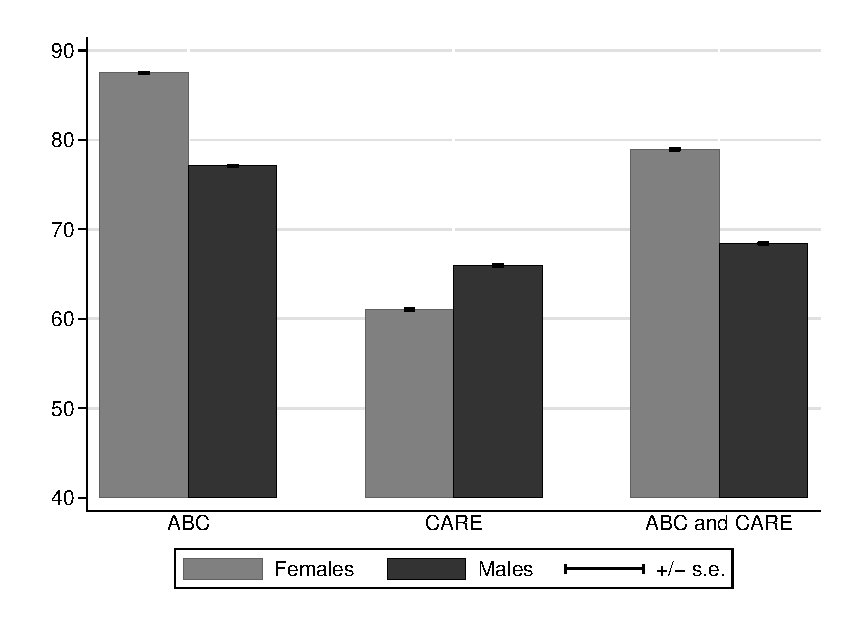
\includegraphics[width=.7\columnwidth]{output/itt_noctrl_all.eps}
\floatfoot{
\footnotesize
\noindent Note: The bars compare the mean of positive impacted outcomes between subjects in ABC/CARE who received center-based childcare and subjects who received no treatment at all.}
\end{figure}

\begin{figure}[H]
		\caption{Positively Impacted Outcomes by Category, ABC/CARE Males and Females} \label{fig:ppositivecategory1}
		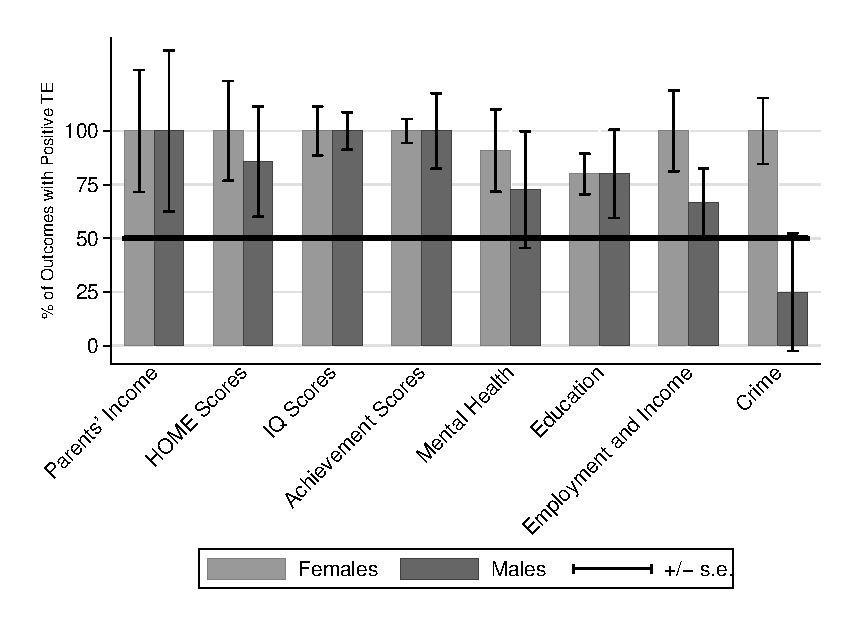
\includegraphics[width=.65\columnwidth]{output/itt_noctrl_cats1.eps}
\floatfoot{
\footnotesize
\noindent Note: For each outcome category, we compare the mean of the subjects who received center-based childcare in ABC/CARE to the mean of the subjects in the control group and count the number of positive comparisons.}
\end{figure}

\begin{figure}[H]
		\caption{Positively Impacted Health Outcomes, ABC/CARE Males and Females} \label{fig:ppositivecategory2}
		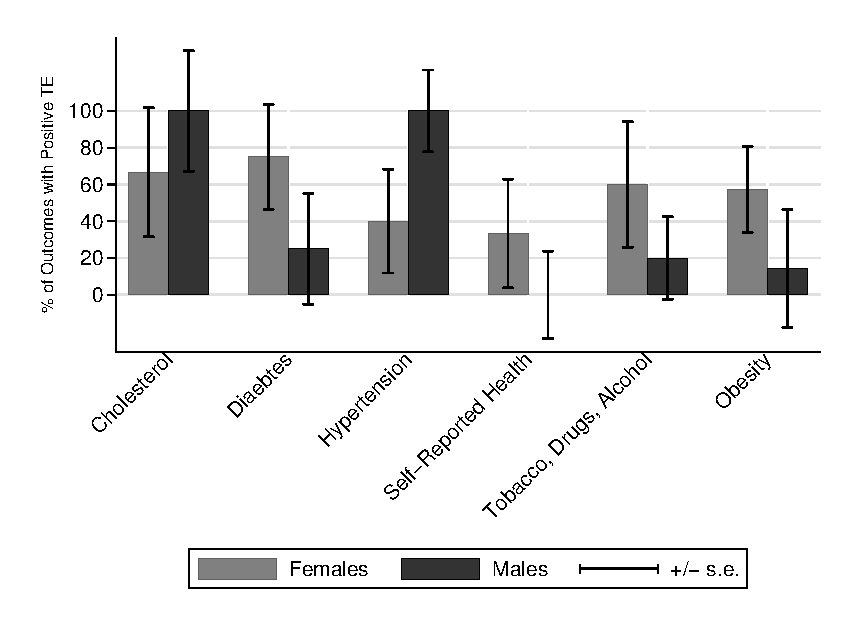
\includegraphics[width=.65\columnwidth]{output/itt_noctrl_cats2.eps}
\floatfoot{
\footnotesize
\noindent Note: For each outcome category, we compare the mean of the subjects who received center-based childcare in ABC/CARE to the mean of the subjects in the control group and count the number of positive comparisons.}
\end{figure}

\section{Cost/benefit Analysis} \label{section:cbaresults}

\subsection{Program Costs} \label{section:programscosts}

The yearly cost of the program was \$18,514 per participant in 2014 USD. We improve on previous cost estimates using primary-source documents.\footnote{These are progress reports written by the principal investigators and related documentation recovered in the archives of the research center where the program was implemented. We display these sources in Appendix \ref{app:programcosts}. Wages are adjusted upward by 15\% to account for fringe benefits. The costs we label as ``other'' arise from nutrition and services that the subjects received when they were sick, diapers during the first 15 months of their lives, and transportation to the center. The control children also received diapers during approximately 15 months, and iron-fortified formula. We assume that this generated a cost that amounts to half of the ``other'' category for the first 15 months of their lives. The costs are based on sources describing ABC treatment for $52$ children. We use the same costs estimates for CARE, for which information is less available. The costs exclude any expenses related to research or policy analysis. Our calculation of the costs per year in 1979 USD is $\$295,239$. A separate calculation of the program as implemented indicates that the yearly cost of the program was $\$275,475$ (1979 USD). See Appendix \ref{app:programcosts}.}

\subsection{Non-experimental Data Sources}

To construct cost-benefit estimates we (i) \textit{interpolate} components not observed due to intermittent data collection; and (ii) \textit{extrapolate} (forecasting) components not observed because the follow-ups stop when the subjects were in their mid-30s. We use multiple sources of non-experimental data representative on the national or state level to construct these interpolations and extrapolations. Table~\ref{table:sources} presents the components for which we do these exercises and the sources we use. Figure~\ref{fig:control-sub} shows the quality of the interpolation and extrapolation of labor income by comparing the forecasts in the ABC/CARE data with the life-cycle profile of disadvantaged individuals in the PSID. Section~\ref{section:methodology} explains our methodology for doing so.

\begin{table}[H]
\begin{threeparttable}
\caption{Auxiliary Data Sources for Interpolation and Extrapolation of Life-cycle Benefits and Costs} \label{table:sources}
\footnotesize
%\input{../../AuxilliaryFiles/Preamble}
%\newgeometry{margin=.1in}

%\newcolumntype{L}[1]{>{\raggedright\let\newline\\\arraybackslash\hspace{0pt}}m{#1}}
%\newcolumntype{C}[1]{>{\centering\let\newline\\\arraybackslash\hspace{0pt}}m{#1}}
%\newcolumntype{R}[1]{>{\raggedleft\let\newline\\\arraybackslash\hspace{0pt}}m{#1}}

\begin{tabular}{L{3cm} C{1cm} C{1cm} C{1cm} C{1cm} C{1cm} C{2cm}} \toprule
 & \multicolumn{6}{c}{Subject's Age} \\
\textbf{Component}  & 16--20 & 21--30 & 31--34 & 35--50 & 51--67 & 68--Death \\ \midrule
\textbf{Transfer Income} & & \multicolumn{1}{c}{\cellcolor[gray]{.8} CNLSY} & \multicolumn{3}{c}{\cellcolor[gray]{.7} NLSY79; PSID}  &  \\ \midrule
\textbf{Subject Income} & &  \multicolumn{1}{c}{\cellcolor[gray]{.8} CNLSY} & \multicolumn{3}{c}{\cellcolor[gray]{.7} NLSY79; PSID} & \\ \midrule
\textbf{Health}  & \multicolumn{6}{c}{\cellcolor[gray]{.8} PSID; MEPS; MCBS; HRS}     \\ \midrule
\textbf{Crime} & \multicolumn{4}{c}{\cellcolor[gray]{.8} NCDPS; NJRP; NVS; UCRS} \\ \bottomrule
\end{tabular}
%\end{document}
\begin{tablenotes}
\footnotesize
Note: This table details the non-experimental data sources we use to interpolate and extrapolate the life-cycle benefits and costs of ABC/CARE. cNLSY: Children of the National Longitudinal Survey of the Youth 1979; NLSY79: National Longitudinal Survey of the Youth 1979; PSID: Panel Study of Income Dynamics; MEPS: Medical Expenditure Panel Survey; MCBS: Medicare Current Beneficiary Survey; HRS: Health and Retirement Study; NCDPS: North Carolina Department of Public Safety Data; NVS: National Crime Victimization Survey; NJRP: National Judicial Reporting Program; UCRS: Uniform Crime Reporting Statistics.
\end{tablenotes}
\end{threeparttable}
\end{table}

\begin{sidewaysfigure}[H]
\centering
\caption{Labor Income Profiles}\label{fig:labor-income-profiles}
\begin{subfigure}[h]{0.4\textwidth}
		\centering
		\caption{Forecasted for ABC/CARE Males} \label{fig:abcare1}
		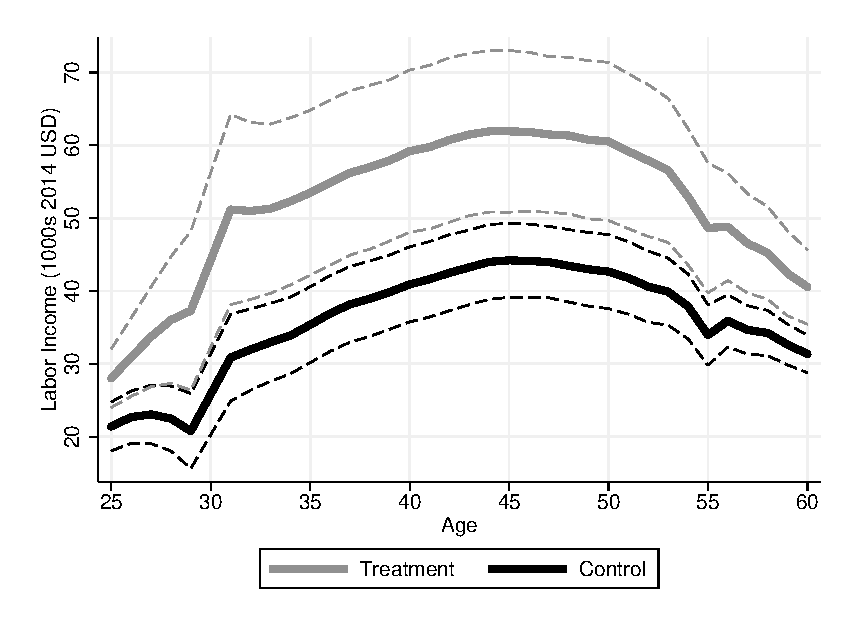
\includegraphics[width=\textwidth]{output/labor_25-60_male.eps}
\end{subfigure}%
\begin{subfigure}[h]{0.4\textwidth}
	\centering
	\caption{PSID, Disadvantaged Males} \label{fig:psid1}
		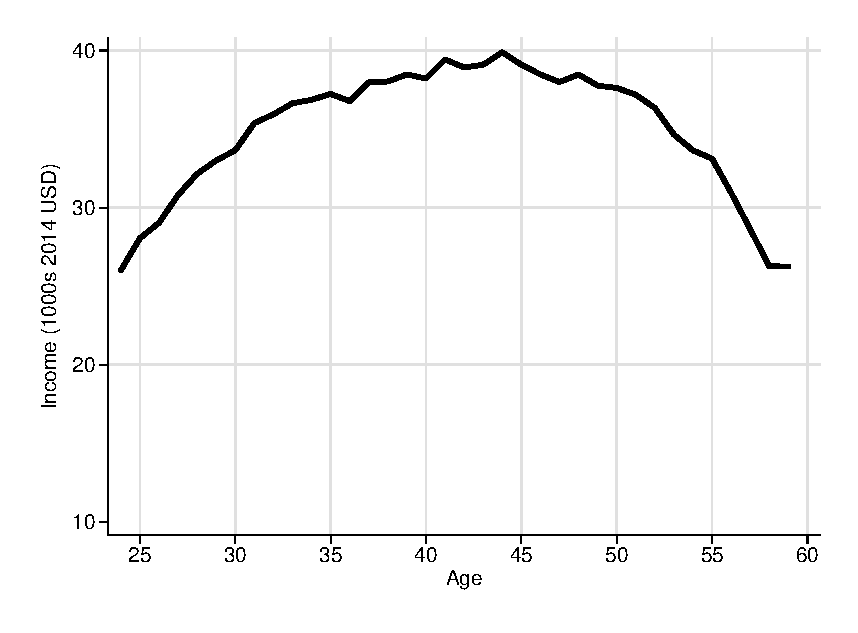
\includegraphics[width=\textwidth]{output/psid_incomeprofiles_s1.eps}
\end{subfigure}
\begin{subfigure}[h]{0.4\textwidth}
		\centering
		\caption{Forecasted for ABC/CARE Females} \label{fig:abcare0}
		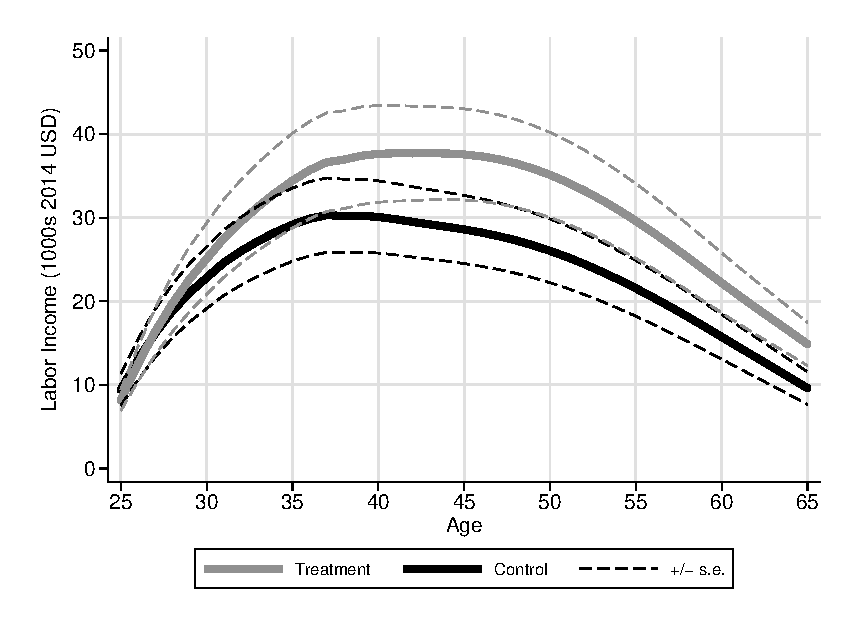
\includegraphics[width=\textwidth]{output/labor_25-60_female.eps}
\end{subfigure}%
\begin{subfigure}[h]{0.4\textwidth}
	\centering
	\caption{PSID, Disadvantaged Females} \label{fig:psid0}
		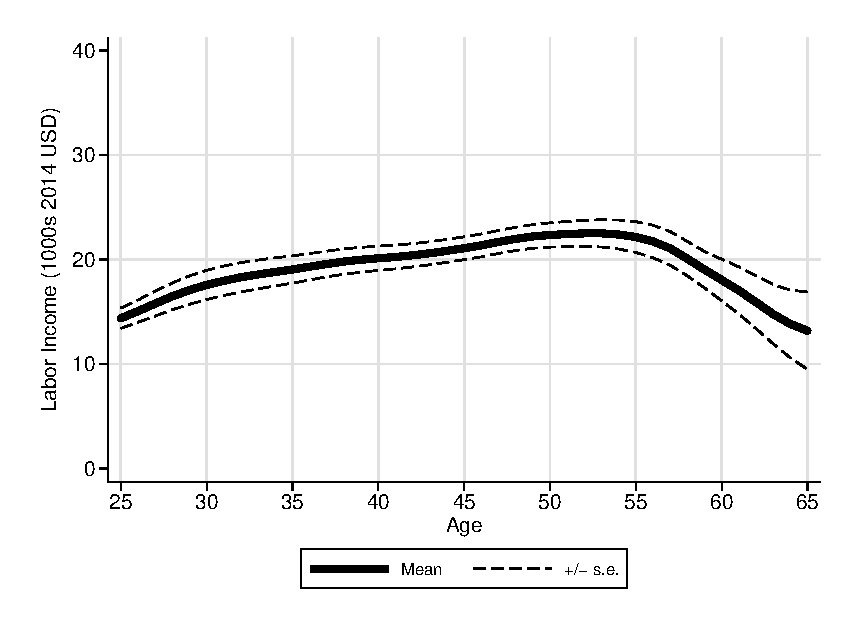
\includegraphics[width=\textwidth]{output/psid_incomeprofiles_s0.eps}
\end{subfigure}
\footnotesize \justify
Note: Panels (a) and (c) display the forecasted labor income profiles for ABC/CARE males and females by treatment status, based on forecasts that combine data from the Panel Study of Income Dynamics (PSID), the National Longitudinal Survey of Youth 1979 (NLSY79), and the Children of the National Longitudinal Survey of Youth 1979 (cNLSY79). Panels (b) and (d) display the median labor income profile of disadvantaged males females in the Panel Study of Income Dynamics (PSID), where disadvantaged is defined as having 12 years of education or less.
\end{sidewaysfigure}


Figure~\ref{figure:npvs} presents the net present values for the main components of the cost/benefit analysis pooling males and females. The ``Baseline'' bars represent the estimates based on the first parameter of interest, comparing the treatment- to the control-group subjects. The ``Stay at Home'' bars represent the comparison between the treatment-group and the control-group subjects who stayed at home. The ``Alternative Preschool'' bars represent the comparison between the treatment-group and the control-group subjects who attended alternative preschools.

The first category, ``Costs," represents the cost of the programs' implementation. The second category, ``Total Net Benefits" quantifies the benefits for the treatment-group subjects net of the benefits of the control-group subjects. Labor income has two components, ``Labor Income" and ``Parental Income." The program produces a positive net present value on labor income of the treated subjects. This considers the income from age 21 all the way to retirement. However it is important to account for the fact that the parents of the treatment-group subjects increased their labor supply and therefore their income. The net present value of parental income span the first 15 years of the treatment and control children.

Crime is an important component, which is consistent with previous analysis of early childhood education programs.\footnote{\citet{Heckman_Moon_etal_2010_RateofReturn}.} We then present two main categories for health, ``QALYs" and ``Medical Costs." As documented in \citet{Campbell_Conti_etal_2014_EarlyChildhoodInvestments}, ABC/CARE had substantial effects on several measures of long-term health, especially for males---e.g. body-mass index, systolic and diastolic pressure, Framigham risk index. This translates into a higher probability of survival at later ages. Thus, individuals in the treatment group incur higher medical costs. However, their health conditions enable them to lead higher quality lives, which is reflected in the net gain the program generates in the QALYs. Finally, we present the net present value of education costs. It is negative because subjects in the treatment group acquired more education throughout their life cycles.

It is important to note that although the net present values from the three comparisons imply that ABC/CARE is socially beneficial regardless of control substitution, the magnitudes for some of the components do vary substantially. We argue that this has to do with the differential treatment effects of ABC/CARE by gender. As Figure~\ref{figure:npvsf} and Figure~\ref{figure:npvsm} show, males benefit much more when the counterfactual scenario is to attend alternative preschools, while females benefit much more from the program when the counterfactual scenario is to stay at home.

\begin{sidewaysfigure}[H]
\caption{Life-cycle Net Present Value of Main Components of the CBA, Pooled Sample of Males and Females}
\label{figure:npvs}
\centering
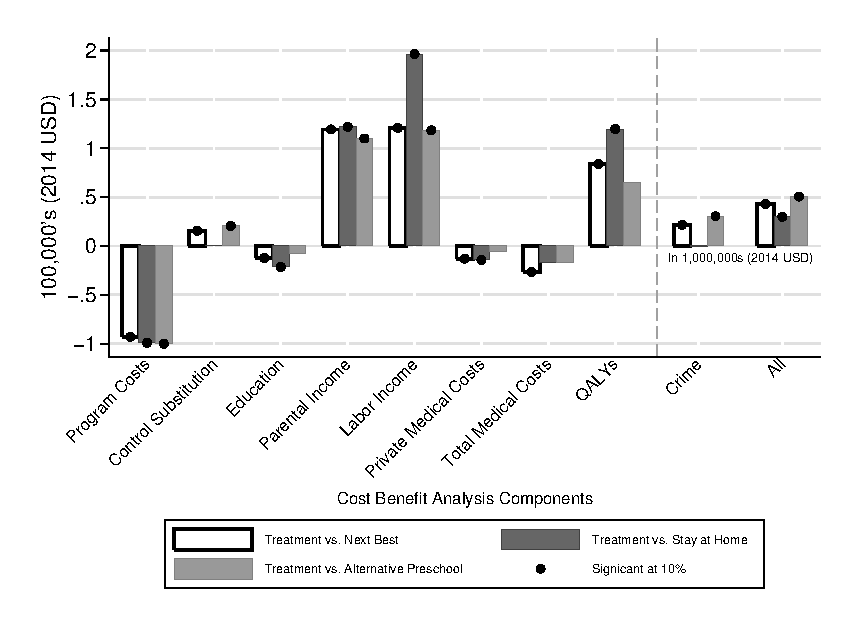
\includegraphics[width=.7\columnwidth]{output/abccare_npvs3.eps}
\floatfoot{
\footnotesize
Note: This figure displays the life-cycle net present values of the main components of the cost/benefit analysis of ABC/CARE from birth to age 79, discounted to birth at a rate of 3\%. ``Treatment vs. Control'': compares the treatment to the control group. ``Treatment vs. Stay at Home'': compares the treatment group to those subjects who stayed at home. ``Treatment vs. Alternative Preschool'': compares the treatment group to those subjects who attended alternative preschools. The latter two are based on matching estimators that account for selection on observable variables. By ``net" we mean that each component represents the total value for the treatment group minus the total value for the control group. Program costs: the total cost of implementing ABC/CARE. Total net benefits: the total net benefits of \textit{all} the components we consider. Labor income: total individual labor income from ages 20 to the retirement of program participants. Parental income: total parental labor income of the parents of the program participants from when the participants were ages 0 to 15. Crime: the total cost of crime (judicial and victimization costs). Total medical costs: both private and public medical costs from ages 15 to 79. Costs of education: the total costs of education of the individual from ages 6 to 26 and include any costs from special education and grade retention. \\
*QALYs refers to the quality-adjusted life years gain due to better health conditions through age 79.\\
}
\end{sidewaysfigure}

\begin{sidewaysfigure}[H]
\caption{Life-cycle Net Present Value of Main Components of the CBA, Females}
\label{figure:npvsf}
\centering
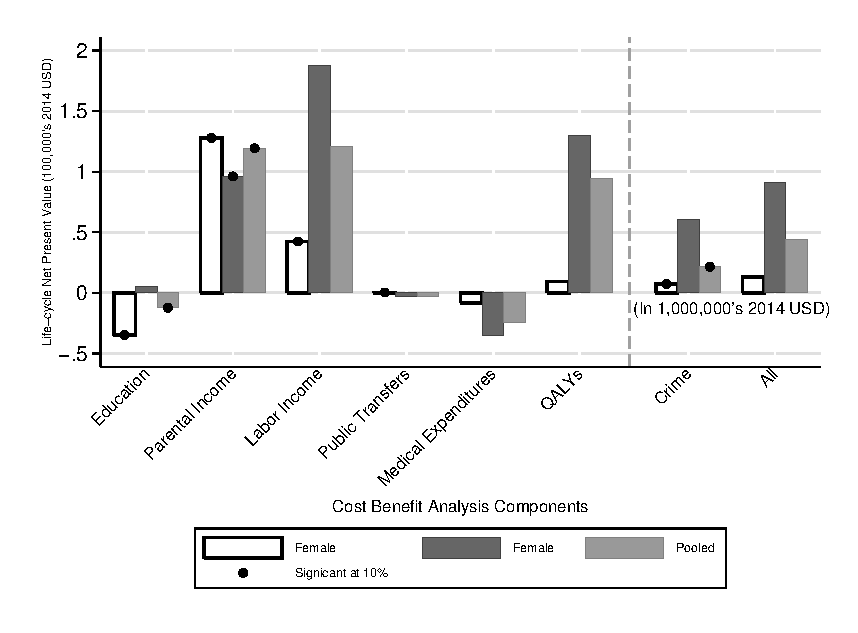
\includegraphics[width=.7\columnwidth]{output/abccare_npvs1.eps}
\floatfoot{
\footnotesize
Note: This figure displays the life-cycle net present values of the main components of the cost/benefit analysis of ABC/CARE from birth to age 79, discounted to birth at a rate of 3\%. ``Treatment vs. Control'': compares the treatment to the control group. ``Treatment vs. Stay at Home'': compares the treatment group to those subjects who stayed at home. ``Treatment vs. Alternative Preschool'': compares the treatment group to those subjects who attended alternative preschools. The latter two are based on matching estimators that account for selection on observable variables. By ``net" we mean that each component represents the total value for the treatment group minus the total value for the control group. Program costs: the total cost of implementing ABC/CARE. Total net benefits: the total net benefits of \textit{all} the components we consider. Labor income: total individual labor income from ages 20 to the retirement of program participants. Parental income: total parental labor income of the parents of the program participants from when the participants were ages 0 to 15. Crime: the total cost of crime (judicial and victimization costs). Total medical costs: both private and public medical costs from ages 15 to 79. Costs of education: the total costs of education of the individual from ages 6 to 26 and include any costs from special education and grade retention. \\
*QALYs refers to the quality-adjusted life years gain due to better health conditions through age 79.\\
}
\end{sidewaysfigure}

\begin{sidewaysfigure}[H]
\caption{Life-cycle Net Present Value of Main Components of the CBA, Males}
\label{figure:npvsm}
\centering
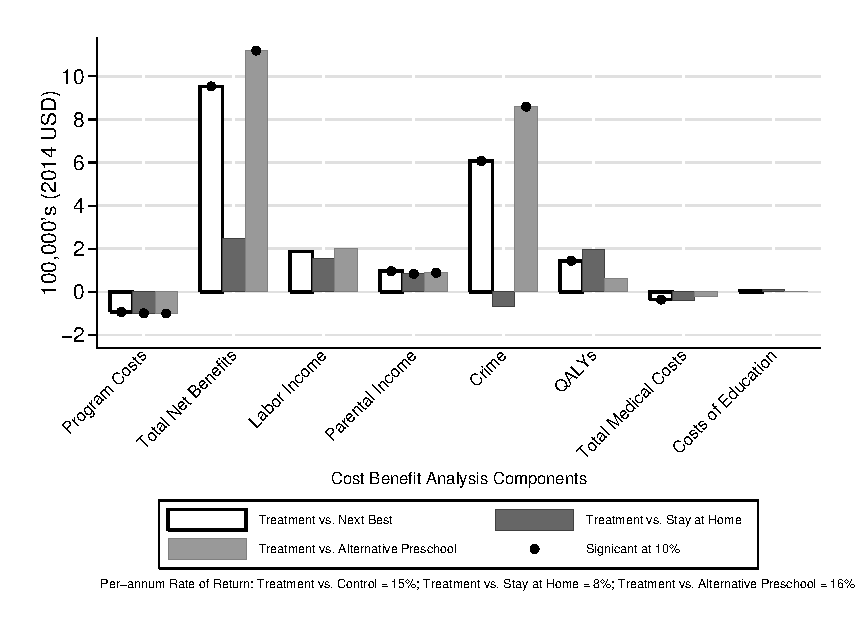
\includegraphics[width=.7\columnwidth]{output/abccare_npvs2.eps}
\floatfoot{
\footnotesize
Note: This figure displays the life-cycle net present values of the main components of the cost/benefit analysis of ABC/CARE from birth to age 79, discounted to birth at a rate of 3\%. ``Treatment vs. Control'': compares the treatment to the control group. ``Treatment vs. Stay at Home'': compares the treatment group to those subjects who stayed at home. ``Treatment vs. Alternative Preschool'': compares the treatment group to those subjects who attended alternative preschools. The latter two are based on matching estimators that account for selection on observable variables. By ``net" we mean that each component represents the total value for the treatment group minus the total value for the control group. Program costs: the total cost of implementing ABC/CARE. Total net benefits: the total net benefits of \textit{all} the components we consider. Labor income: total individual labor income from ages 20 to the retirement of program participants. Parental income: total parental labor income of the parents of the program participants from when the participants were ages 0 to 15. Crime: the total cost of crime (judicial and victimization costs). Total medical costs: both private and public medical costs from ages 15 to 79. Costs of education: the total costs of education of the individual from ages 6 to 26 and include any costs from special education and grade retention. \\
*QALYs refers to the quality-adjusted life years gain due to better health conditions through age 79.\\
}
\end{sidewaysfigure}

We analyze the internal rate of return and cost-benefit ratio implied by the net present values presented in Figure~\ref{figure:npvs} through Figure~\ref{figure:npvsm}. These results without accounting for control substitution are presented in Table~\ref{table:cba}. All the monetary figures are in 2014 USD and are discounted to each child's birth.

Pooling males and females, the results indicate that the program is socially efficient: the baseline estimates for the internal rate of return and the benefit-to-cost ratio are \irrp\ and \bcp. The program generates a benefit of \bcp\ for every dollar spent on it. This is of particular importance because ABC/CARE was much more expensive than other early childhood education programs---the treatment involved more services over a longer time period \citep{Elango_Hojman_etal_2016_Early-Edu}.

The internal rate of return and the benefit/cost ratio are robust to sensitivity exercises. First, we remove the component due to parental income. In practice, ABC/CARE had a childcare subsidy component because it allowed the mothers to work causing additional parental income. This component amounts to \parincomenpvp. Even after removing this component, the internal rate of return and benefit/cost ratio indicate social efficiency of the program and remain statistically significant.

Parental income and crime are the components for which the internal rate of return and the benefit/cost ratio are the most sensitive.\footnote{We do not account for treatment effects on parental income beyond age 15 because some subjects report to move out of their households as early as this age. This makes ambiguous the effects that parental income could have on the subjects after age 15.} The reason for the sensitivity to parental income is that the amount is substantial and it is not heavily discounted because it accumulates during the first $15$ years of the children's life. Although crime is subject to more discounting, the amount due to crime savings is large so removing it diminishes both the internal rate of return and the benefit-to-cost ratio.

The estimates are robust to individually removing the rest of the components, and in most cases remain statistically significant. This happens for one of either two reasons: (i) the effects are substantial but they are heavily discounted because they happen later in life---e.g. labor income; or (ii) the effects happen early in life but are not as substantial---as in the amount that the control-group parents pay for their children to attend alternative preschools.

Next, we analyze the estimates when splitting the sample by males and females. Some of the estimates lose significance due to the reduction of observations after splitting the sample by gender. The point estimates remain robust across  the sensitivity analysis (see Table~\ref{table:cba}), which computes the benefit/cost ratio and the internal rate of return when removing a component. For females, we observe consistency except for the case where we remove the parental income component. We can observe that the female sample is the main driver of parental income when comparing its net present value between females and males. For males, the estimates are robust, similar to the female sample.

\begin{table}[H]
\centering
\caption{Cost/benefit Analysis of ABC/CARE, Summary}\label{table:cba}
\begin{adjustbox}{max width=\textwidth}
\begin{threeparttable}
\begin{tabular}{l r r r r r r r r r}																			
\toprule																			
&       \mc{3}{c}{Females}      &       \mc{3}{c}{Males}        &       \mc{3}{c}{Pooled}       \\																			
\cmidrule(lr){2-4}      \cmidrule(lr){5-7}      \cmidrule(lr){8-10}																			
Removed Component       &       NPV     &       IRR     &       B/C     &       NPV     &       IRR     &       B/C     &       NPV     &       IRR     &       B/C     \\																			
\midrule																			
None	&		&	0.15	&	\textbf{3.38}	&		&	-.10	&	6.75	&		&	0.10	&	\textbf{4.75}	\\
	&		&	(0.11)	&	(1.59)	&		&	(0.11)	&	(6.22)	&		&	(0.10)	&	(2.04)	\\ \\
Parental Income	&	\textbf{158,017}	&	0.05	&	1.72	&	45,511	&	-.10	&	6.27	&	\textbf{74,718}	&	0.08	&	\textbf{3.96}	\\
	&	(43,586)	&	(0.05)	&	(1.49)	&	(45,289)	&	(0.10)	&	(6.10)	&	(25,250)	&	(0.07)	&	(2.05)	\\
Subject QALY	&	0	&	0.15	&	\textbf{3.38}	&	0	&	-.10	&	6.75	&	0	&	0.10	&	\textbf{4.75}	\\
	&	(0.00)	&	(0.11)	&	(1.59)	&	(0.00)	&	(0.11)	&	(6.22)	&	(0.00)	&	(0.10)	&	(2.04)	\\
Subject Labor Income	&	44,201	&	0.16	&	\textbf{2.92}	&	124,655	&	-.06	&	5.44	&	93,992	&	-.08	&	\textbf{3.76}	\\
	&	(151,724)	&	(0.10)	&	(0.78)	&	(639,086)	&	(0.10)	&	(4.72)	&	(119,314)	&	(0.09)	&	(1.72)	\\
Subject Transfer Income	&	-1,276	&	0.16	&	\textbf{3.40}	&	-2,318	&	-.10	&	6.78	&	6,255	&	0.10	&	\textbf{4.68}	\\
	&	(34,263)	&	(0.11)	&	(1.60)	&	(33,759)	&	(0.11)	&	(6.23)	&	(9,411)	&	(0.10)	&	(2.04)	\\
Medical Expenditures	&	14,344	&	0.15	&	\textbf{3.23}	&	14,905	&	\textbf{0.13}	&	6.59	&	14,645	&	\textbf{0.10}	&	\textbf{4.60}	\\
	&	(82,883)	&	(0.15)	&	(1.55)	&	(146,935)	&	(0.10)	&	(6.17)	&	(39,129)	&	(0.07)	&	(2.03)	\\
Control Contamination	&	\textbf{19,884}	&	\textbf{0.12}	&	\textbf{3.17}	&	\textbf{15,608}	&	-.10	&	6.59	&	\textbf{15,073}	&	0.09	&	\textbf{4.59}	\\
	&	(3,147)	&	(0.08)	&	(1.59)	&	(2,324)	&	(0.11)	&	(6.21)	&	(2,229)	&	(0.09)	&	(2.03)	\\
Education Costs	&	-47,183	&	0.16	&	\textbf{3.88}	&	15,340	&	-.10	&	6.59	&	-11,353	&	0.11	&	\textbf{4.87}	\\
	&	(14,395)	&	(0.11)	&	(1.58)	&	(13,222)	&	(0.11)	&	(6.23)	&	(11,316)	&	(0.10)	&	(2.06)	\\
Crime Costs	&	\textbf{133,116}	&	0.14	&	1.98	&	427,343	&	0.07	&	2.25	&	\textbf{257,780}	&	0.07	&	2.04	\\
	&	(44,756)	&	(0.10)	&	(1.47)	&	(447,081)	&	(0.09)	&	(3.64)	&	(172,485)	&	(0.06)	&	(1.15)	\\ \\
Deadweight Loss	&		&	0.23	&	\textbf{4.70}	&		&	-.10	&	9.70	&		&	0.13	&	\textbf{6.77}	\\
	&		&	(0.18)	&	(2.36)	&		&	(0.12)	&	(9.36)	&		&	(0.13)	&	(3.04)	\\
0\% Discount Rate	&		&		&	\textbf{7.10}	&		&		&	14.72	&		&		&	\textbf{11.89}	\\
	&		&		&	(4.66)	&		&		&	(15.56)	&		&		&	(5.21)	\\
5\% Discount Rate	&		&		&	\textbf{2.39}	&		&		&	4.29	&		&		&	\textbf{2.81}	\\
	&		&		&	(0.90)	&		&		&	(3.61)	&		&		&	(1.17)	\\
\bottomrule																			
\end{tabular}																			

\begin{tablenotes}
\footnotesize
\item Note: This table presents the estimates of the net present value (NPV) for each component, and the internal rate of return (IRR) and the benefit/cost ratio (B/C) of ABC/CARE for different scenarios based on comparing the groups randomly assigned to receive center-based childcare and the groups randomly assigned as control in ABC/CARE. The first row represents the baseline estimates. The rest of the rows present estimates for scenarios in which we remove the NPV estimates of the component listed in the first column. The quantity listed in the NPV columns is the component we actually remove when computing the calculation in each row. All the money figures are in 2014 USD and are discounted to each child's birth, unless otherwise specified. For the B/C we use a discount rate of $3\%$, unless otherwise specified. We test the null hypotheses $\text{IRR} = 3\%$ and $\text{B/C} = 1$---we elect $3\%$ because that is the discount rate we use. The results in bold are significant at the 10\% level in a single-sided, non-parametric, bootstrapped test. We resample both the experimental and the auxiliary data sources.
\end{tablenotes}
\end{threeparttable}
\end{adjustbox}
\end{table}

We provide a cost-benefit analysis of the program when accounting for control substitution (Table~\ref{table:cbacs}). The first row shows the estimates without accounting for control substitution, i.e. the same as those of the first row in Table~\ref{table:cba}. The second and third rows present results for the two counterfactual comparisons we consider.

The results are consistent with the treatment effects we show in Section~\ref{section:teresults}. Compared to ABC/CARE, females benefit more than males from alternative preschools relative to staying at home. That is, the benefit/cost ratio of ABC/CARE relative to staying at home is high for females and low for males. Conversely, the benefit/cost ratio of ABC/CARE relative to alternative preschools is high for males and low for females. Given the outcomes that we are able to monetize have higher values for males than for females, the pooled results are more similar to the results for males than to the results for females. Regardless, any of the counterfactual comparisons we consider indicates that ABC/CARE is socially efficient.

\begin{table}[H]
\begin{threeparttable}
\caption{Cost/benefit Analysis Accounting for Control Substitution}
\label{table:cbacs}
\centering
\begin{tabular}{l c c c c c c }
\toprule
	&	\mc{2}{c}{Females}					&	\mc{2}{c}{Males}					&	\mc{2}{c}{Pooled}					\\
		\cmidrule(lr){2-3}						\cmidrule(lr){4-5}						\cmidrule(lr){6-7}					
Estimate 	&	IRR	&	B/C	&	IRR	&	B/C	&	IRR	&	B/C	\\
\midrule

% INSERT summary_tex.xls FILE BELOW
% INSERT summary_tex.xls FILE BELOW
% INSERT summary_tex.xls FILE BELOW

Baseline	&	0.09 	&	\textbf{2.53}	&	\textbf{0.14} &	\textbf{9.75} 	&	\textbf{0.13}	&	\textbf{5.56}	\\
	&	(0.05)	&	(0.97)	&	(0.05)	&	(4.64)	&	(0.05)	&	(2.39)	\\
Relative to Staying at Home	&	\textbf{0.13}	&	\textbf{4.77}	&	\textbf{0.08}	&	4.38	&	\textbf{0.10} &	\textbf{4.41}	\\
	&	(0.05)	&	(1.40)	&	(0.04)	&	(2.65)	&	(0.03)	&	(1.34)	\\
Relative to Alternative Preschools	&	0.09		&	\textbf{2.30}	&	\textbf{0.16}	&	\textbf{12.48}	&	\textbf{0.13}	&	\textbf{6.22}	\\
	&	(0.06)	&	(0.90)	&	(0.04)	&	(5.13)	&	(0.04)	&	(2.23)	\\

% INSERT summary_tex.xls FILE ABOVE
% INSERT summary_tex.xls FILE ABOVE
% INSERT summary_tex.xls FILE ABOVE

\bottomrule
\end{tabular}
\begin{tablenotes}
\footnotesize
\item Note: This table displays estimates of the internal rate of return (IRR) and the benefit-to-cost ratio (B/C) for ABC/CARE for three cases. Not accounting for control substitution (baseline); comparing ABC/CARE to staying at home (relative to staying at home); and comparing ABC/CARE to alternative preschools (relative to alternative preschools). For the B/C we use a discount rate of $3\%$. We test the null hypotheses $\text{IRR} = 3\%$ and $\text{B/C} = 1$---we elect $3\%$ because that is the discount rate we use. The results in bold are significant at the 10\% level in a single-sided, non-parametric, bootstrapped test. We resample both the experimental and the auxiliary data sources.
\end{tablenotes}
\end{threeparttable}
\end{table}

\subsection{Using our Estimates to Understand Recent Cost/benefit Analyses}

\noindent An example of the approach recent studies take on cost-benefit analyses is \citet{Kline-Walters_2016_QJE}. They use data of the Head Start Impact Study (HSIS) to evaluate Head Start and find that a benefit/cost ratio between $1.50$ and $1.84$.\footnote{HSIS is a one-year-long randomized evaluation of Head Start.} Their analysis contains three steps: (i) calculate the treatment effect on Wechsler Preschool and Primary Scale of Intelligence (WPPSI) at age 5; (ii) monetize this gain using the return to WPPSI at age 5 in terms of net present value of labor income at age 27 \citep{Chetty_Friedman_etal_2011_QJoE}.\footnote{For this exercise, we interpret the earnings estimated in \citet{Chetty_Friedman_etal_2011_QJoE} to be equivalent to labor income.} Calculations from \citet{Chetty_Friedman_etal_2011_QJoE} indicate that a 1 standard deviation gain in WPPSI at age 5 implies a $13.1\%$ increase in the net present value of labor income at age 27;\footnote{This is based on combining information from Project Star and administrative data at age 27.} and (iii) calculate the benefit/cost ratio based on this gain and their own calculations of the program's cost. This calculation is based on assigning the net present value of labor income at age 27 of $\$385,907.17$ to the control-group participants, which is provided by  \citet{Chetty_Friedman_etal_2011_QJoE}.\footnote{All money values that we provide in this section are in 2014 USD.}


\begin{table}[H]
\begin{threeparttable}
\caption{Alternative Cost-benefit Analyses Calculations}
\label{table:comparing}
\centering
\footnotesize

\begin{tabular}{cllcc}
\toprule
Age & \mc{1}{c}{NPV Source} & Component & \citet{Kline-Walters_2016_QJE} & Authors' Method \\
& & & Method & \\
\midrule
\multirow{2}{*}{27} & \cite{Chetty_Friedman_etal_2010_HowDoesYour} & Earnings & 1.04 (s.e. 0.36) &  \\
& ABC/CARE-calculated & Earnings & 1.36 (s.e. 0.04) &  0.14 (s.e. 0.05)\\
\midrule
\multirow{2}{*}{34} & ABC/CARE-calculated & Earnings & 0.45 (s.e. 0.04) & 0.45 (s.e. 0.17) \\
& ABC/CARE-calculated & All & 0.88 (s.e. 0.04) &  0.88 (s.e. 0.34) \\
\midrule
\multirow{2}{*}{Life-cycle} &  ABC/CARE-calculated & Earnings & 1.58 (s.e. 0.07) & 1.58 (s.e. 0.60) \\
& ABC/CARE-calculated & All & 4.58 (s.e. 0.25) & 5.63 (s.e. 2.15) \\
\bottomrule
\end{tabular}

\begin{tablenotes}
\footnotesize
\item Note: This table displays displays benefit/cost ratios based on the methodology in \citet{Kline-Walters_2016_QJE} and based on our own methodology. Age: age at which we stop calculating the net-present value. NPV Source: source where we obtain the net present value. Component: item used to compute net present value (all refers to the net present value of all the components). \citet{Kline-Walters_2016_QJE} Method: estimate based on these authors methodology. Author's Method: estimates based on our methodology.
\end{tablenotes}
\end{threeparttable}
\end{table}

To analyze how our estimates compares to the method in \citet{Kline-Walters_2016_QJE}, we present a series of exercises in the third column of Table~\ref{table:comparing}. For comparison, the fourth column of Table~\ref{table:comparing} displays the analogous exercise using our own method.

In the first exercise, we use both the ``return to WPPSI'' and the net-present value of labor income at age 27 in  \citet{Chetty_Friedman_etal_2011_QJoE}. In the second exercise, we perform a similar exercise but we use our own estimate of the net-present value of labor income at age 27.\footnote{This allows us to compute our own ``return to WPPSI'' and impute it to the treatment-group individuals.} The reminder of exercises are similar, but (i) vary the age up to where we consider the net-present value of labor income; (ii) consider the value of all the components we analyze throughout the paper; or (iii) both.

Our methodology has three gains: (i) provides a more precise estimate of the net-present value (and the return to WPPSI) of the components, as our interpolation and extrapolation are based on matching our experimental sample to various non-experimental samples. We do not impute a net present value or a return of an \textit{ad hoc} experiment; (ii) we better quantify the effects of the analyzed experiment by considering the whole life-cycle; and (iii) we better approximate the statistical uncertainty of our estimates by considering both the sampling error in the experimental and non-experimental samples and the forecasting error due to the interpolation and extrapolation.

\section{Summary} \label{section:conclusion}

The statistical evidence about the effectiveness of early childhood education is scarce. We evaluate two randomized controlled trials: the Carolina Abecedarian Project (ABC) and the Carolina Approach to Responsive Education (CARE).

As programs providing high-quality center-based childcare, ABC/CARE has positive effects on a variety of outcomes measuring human development throughout childhood to adulthood---including cognition, socio-emotional skills, criminal activity, and adulthood health. This translates into statistically and economically significant measures of social efficiency, like the benefit-cost ratio and the internal rate of return, which we calculate accounting for complications that arise when evaluating social programs and considering life-cycle gains.

When adequately assessed, early childhood education programs enhance human development in that they provide a vehicle to promote social mobility. An adequate evaluation requires: (i) comparing the program with respect to a well-defined counterfactual---e.g. other programs or staying at home; and (ii) monetizing the life-cycle gains, which goes beyond back-of-the-envelope calculations based on short-term gains.

\clearpage

%References
\singlespace
\bibliographystyle{chicago}
\bibliography{heckman}

\end{document} 